% !TEX root = ../OT4ML.tex

\chapter{Wasserstein Gradient Flows}
\index{Wasserstein!gradient}% strictindex
\index{gradient!flow}% strictindex
\index{Wasserstein!gradient flow}% strictindex
\label{sec-wasserstein-gradient-flows}

Once $\Wass_2$ is a dynamic metric, one can run gradient descent directly on the space of measures. This chapter derives the formal Wasserstein gradient, explains the JKO minimizing-movement scheme, records the role of geodesic convexity in convergence, and then applies the same calculus to mean-field neural-network training.
\index{mean-field neural network}% strictindex
\index{minimizing movement scheme}% strictindex
\index{convexity!geodesic}% strictindex
\index{JKO scheme}% strictindex

\section{Minimizing Movements and Wasserstein Gradients}
\index{minimizing movement}% strictindex
\index{Wasserstein!gradient}% strictindex

This first section explains how a variational implicit-Euler step on measures gives rise, in the small-step limit, to a continuity equation driven by the Wasserstein gradient of the energy.
\index{continuity equation}% strictindex

We now consider a function $f(\alpha)$ and seek a minimizing evolution $(\alpha_t)_t$. The general strategy of minimizing movement over a metric space is to construct a discrete-time evolution using an implicit Euler scheme:
\index{implicit Euler scheme}% strictindex
\begin{equation}
    \alpha_{t+\tau} := \arg\min_\alpha \frac{1}{2 \tau} \Wass_2(\alpha_t, \alpha)^2 + f(\alpha). \label{eq:jko-discr}
\end{equation}


\paragraph{Euclidean gradient flows.}
\index{gradient!flow}% strictindex

If we restrict \eqref{eq:jko-discr} to finite dimensions and assume $\alpha_t = \delta_{x(t)}$ and $\alpha = \delta_x$ (single Dirac measures), this matches the implicit Euler scheme:
\index{Dirac mass}% strictindex
\index{implicit Euler scheme}% strictindex
\begin{equation*}
    x(t+\tau) := \arg\min_x \frac{1}{2 \tau} \norm{x - x(t)}^2 + h(x),
\end{equation*}
where $h(x) = f(\delta_x)$. Its solution is formally given by the implicit Euler formula:
\begin{equation*}
    x(t+\tau) = (\Id + \tau \nabla h)^{-1}(x(t)).
\end{equation*}
In contrast, the explicit Euler scheme is:
\begin{equation*}
    x(t+\tau) = (\Id - \tau \nabla h)(x(t)) = x(t) - \tau \nabla h(x(t)).
\end{equation*}

Both schemes converge as $\tau \to 0$ to:
\begin{equation}
    \dot{x}(t) = -\nabla h(x(t)). \label{eq:grad-flow-classical}
\end{equation}


\paragraph{Wasserstein gradient formula.}
\index{Wasserstein!gradient}% strictindex

The implicit Euler scheme has the advantage that it does not require $h$ or $f$ to be smooth. For $f$, this is crucial to handle evolutions over measures that may have densities, atoms or other singular parts.
\index{implicit Euler scheme}% strictindex

As $\tau \to 0$, under certain conditions on $f$, \eqref{eq:jko-discr} defines a continuous evolution $t \mapsto \alpha_t$. As discussed earlier, this evolution can be described as a Lagrangian evolution \eqref{eq:lagrangian-advection}. We use the following first-variation convention: for any $\beta\in\Pp(\RR^d)$ and the signed zero-mass perturbation $\rho=\beta-\alpha$,
\index{first variation}% strictindex
\index{signed!measure}% strictindex
\begin{equation*}
    f((1-\tau)\alpha + \tau \beta) = f(\alpha + \tau \rho) = f(\alpha) + \tau \int [\delta f(\alpha)](x) \d \rho(x) + o(\tau).
\end{equation*}
The key infinitesimal object is the vector field that represents this differential in the Wasserstein metric.

\begin{defn}[Wasserstein gradient]\label{def-wasserstein-gradient}
\index{Wasserstein!gradient}% strictindex
	Assume that $f$ admits a smooth first variation $\delta f(\alpha)$. In the smooth formal calculus on $\Pp_2(\RR^d)$, the Wasserstein gradient of $f$ at $\alpha$ is the gradient vector field
	\begin{equation*}
	    \Wgrad f(\alpha) = \nabla_x \delta f(\alpha).
	\end{equation*}
\end{defn}
The associated formal gradient flow is the continuity equation
\begin{equation}
    \frac{\partial \alpha_t}{\partial t} + \diverg(-\Wgrad f(\alpha_t) \alpha_t) = 0. \label{eq:wassflow-pde}
\end{equation}
The following proposition explains why this vector field is the Riemannian gradient for the $L^2(\alpha)$ metric on velocities.
\index{signed!measure}% strictindex
%
\begin{proposition}[Formal Wasserstein gradient]\label{prop-formal-wass-gradient}
\index{Wasserstein!gradient}% strictindex
	Assume that $f$ admits a smooth first variation $\delta f(\alpha)$ and that $\alpha$ has a smooth positive density. For infinitesimal perturbations generated by a velocity field $v$ through $(\Id+\tau v)_\sharp\alpha$, the differential of $f$ is
\index{first variation}% strictindex
\index{velocity field}% strictindex
	\[
		\frac{\d}{\d\tau}_{|\tau=0}
		f\big((\Id+\tau v)_\sharp\alpha\big)
		=
		\int \dotp{\nabla \delta f(\alpha)(x)}{v(x)}\d\alpha(x).
	\]
	Hence, for the Riemannian metric $\norm{v}_{L^2(\alpha)}^2=\int \norm{v}^2\d\alpha$, the Wasserstein gradient is the vector field
\index{Wasserstein!gradient}% strictindex
	\[
		\Wgrad f(\alpha)=\nabla \delta f(\alpha).
	\]
\end{proposition}
\begin{proof}
	The push-forward expansion gives, in the sense of distributions,
\index{push-forward}% strictindex
	\[
		(\Id+\tau v)_\sharp\alpha
		=
		\alpha-\tau\diverg(\alpha v)+o(\tau).
	\]
	Using the definition of the first variation,
\index{first variation}% strictindex
	\[
		f((\Id+\tau v)_\sharp\alpha)
		=
		f(\alpha)-\tau\int \delta f(\alpha)\diverg(\alpha v)\d x+o(\tau).
	\]
	An integration by parts, with either compact support or vanishing boundary flux, gives
\index{flux}% strictindex
	\[
		-\int \delta f(\alpha)\diverg(\alpha v)\d x
		=
		\int \dotp{\nabla\delta f(\alpha)}{v}\d\alpha.
	\]
	By definition of the Riesz representative for the $L^2(\alpha)$ metric, this representative is $\nabla\delta f(\alpha)$.
\end{proof}

The Wasserstein gradient-flow viewpoint already appears in John D. Lafferty's PhD work, published as ``The Density Manifold and Configuration Space Quantization'', under the name ``density manifold''. It was then systematically developed by Otto, who exposed the formal Riemannian structure of this space~\cite{otto2001geometry}. Rigorous metric-space treatments and numerical JKO schemes can be found in~\cite{ambrosio2006gradient,JDB-JKO,2015-Peyre-siims,gallouet2017jko}.
\index{Wasserstein!gradient}% strictindex
\index{Wasserstein!gradient flow}% strictindex
\index{JKO scheme}% strictindex

%%%%
\paragraph{From the JKO step to the velocity field.}
\index{velocity field}% strictindex

A first-order expansion of the JKO step explains why~\eqref{eq:wassflow-pde} uses the vector field $\Wgrad f(\alpha)$. Write \eqref{eq:jko-discr} as a minimization over displacement fields $v$ such that $\alpha = (\Id + \tau v)_\sharp \alpha_t$:
	\[
		\min_{v} \frac{1}{2 \tau} \tau^2 \norm{v}_{L^2(\alpha_t)}^2 + f( (\Id + \tau v)_\sharp \alpha_t ).
	\]
Then we perform a first-order Taylor expansion of this formulation using
	\[
		 (\Id + \tau v)_\sharp \alpha_t =  \alpha_t - \tau \diverg( v \alpha_t ) + o(\tau)
	\]
	\[
		f( (\Id + \tau v)_\sharp \alpha_t ) = f(\alpha_t) - \tau \int \delta f(\alpha_t) \diverg( v \alpha_t ) \d x + o(\tau)
	\]
	\[
		 = f(\alpha_t) + \tau \int \langle \nabla_x \delta f(\alpha_t)(x), v(x) \rangle \d \alpha_t(x) + o(\tau)
	\]
to obtain the following first-order expansion in $\tau$ of the problem minimized in \eqref{eq:jko-discr}
	\[
		 \min_{v} f(\alpha_t) +  \tau \int \Big[ \frac{1}{2} \norm{v(x)}^2 + \langle \Wgrad f(\alpha_t)(x), v(x) \rangle \Big]\d \alpha_t(x) + o(\tau).
	\]
The pointwise minimizer is $v=-\Wgrad f(\alpha_t)$, which gives the velocity in the continuity equation.
\index{continuity equation}% strictindex

\paragraph{Metric derivative and curves of maximal slope.}
\index{metric!derivative}% strictindex
\index{curve of maximal slope}% strictindex
\index{metric!slope}% strictindex

The same descent principle admits a coordinate-free formulation, which is the right language for limits of JKO schemes. Let $(\mathcal X,d)$ be a metric space and let $x:(0,T)\to\mathcal X$ be an absolutely continuous curve. Its metric derivative is
	\[
		|\dot x_t|
		\eqdef
		\lim_{h\to 0}\frac{d(x_{t+h},x_t)}{|h|}
	\]
for a.e. $t$. Equivalently, $|\dot x_t|$ is the smallest $g\in L^1_{\rm loc}(0,T)$ such that $d(x_s,x_t)\leq \int_s^t g(r)\d r$ for all $0<s<t<T$. If $f:\mathcal X\to(-\infty,+\infty]$ is lower semicontinuous, its local metric slope at a point $x$ with $f(x)<+\infty$ is
	\[
		|\partial f|(x)
		\eqdef
		\limsup_{\substack{y\to x\\ y\neq x}}
		\frac{( f(x)-f(y) )_+}{d(x,y)} .
	\]
When this slope is a strong upper gradient for $f$, meaning that $|f(y_t)-f(y_s)|\leq \int_s^t |\partial f|(y_r)|\dot y_r|\d r$ along absolutely continuous curves $y_r$, an absolutely continuous curve $x_t$ is called a curve of maximal slope if it satisfies the energy-dissipation inequality
	\[
		f(x_t)
		+\frac12\int_s^t |\dot x_r|^2\d r
		+\frac12\int_s^t |\partial f|^2(x_r)\d r
		\leq f(x_s),
		\qquad 0\leq s<t.
	\]
This is the metric-space formulation of gradient descent~\cite{ambrosio2006gradient}; the inequality is stable under weak limits, while in smooth Hilbert or Wasserstein settings it is usually saturated. In $\mathcal X=\Pp_2(\RR^d)$ with $d=\Wass_2$, an absolutely continuous curve admits a continuity-equation velocity $v_t$ and satisfies $|\dot\alpha_t|_{\Wass_2}\leq\norm{v_t}_{L^2(\alpha_t)}$, with equality for the minimal velocity. For smooth energies, $|\partial f|(\alpha_t)=\norm{\Wgrad f(\alpha_t)}_{L^2(\alpha_t)}$, so the maximal-slope condition reduces to the velocity-field equation $v_t=-\Wgrad f(\alpha_t)$ derived above. The energy consequences of this viewpoint are used below in Section~\ref{sec-geodesic-convexity}.

We now detail examples of such Wasserstein gradient flows.
\index{Wasserstein!gradient}% strictindex
\index{gradient!flow}% strictindex
\index{Wasserstein!gradient flow}% strictindex

Figure~\ref{fig:gradflow-jko-entropy-steps} shows the same minimizing-movement construction both in density coordinates and through the motion of quantiles.

\begin{figure}[ht]
\centering
\begin{tabular}{@{}cc@{}}
\small density iterates & \small quantile motion \\[-.15em]
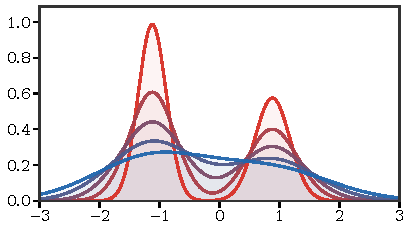
\includegraphics[width=.43\linewidth]{figures/gradflow-jko-entropy-steps--density-steps.pdf} &
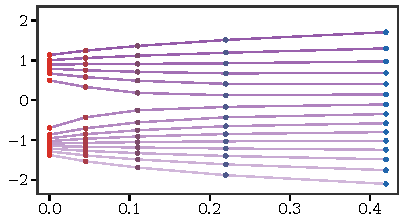
\includegraphics[width=.43\linewidth]{figures/gradflow-jko-entropy-steps--quantile-steps.pdf}
\end{tabular}
\caption{JKO minimizing movements for the entropy flow in one dimension. The left panel displays successive implicit-Euler minimizers for the heat equation, colored from red to blue. The right panel tracks inverse CDF values $Q_t(s)=F_t^{-1}(s)$ for selected probability levels $s$, giving a Lagrangian view of the proximal movement in Wasserstein space.}
\index{minimizing movement}% strictindex
\index{Wasserstein!space}% strictindex
\index{heat equation}% strictindex
\index{JKO scheme}% strictindex
\label{fig:gradflow-jko-entropy-steps}
\end{figure}

%%%
\paragraph{Discrete evolutions.}
\index{measure!evolution}% strictindex

If $f(\alpha)$ can be evaluated on discrete distributions and $\Wgrad$ is continuous in this case, the flow \eqref{eq:wassflow-pde} maintains the number of Dirac masses, $\alpha_t = \frac{1}{n} \sum_i \delta_{x_i(t)}$. The particles $X(t) := (x_i(t))_i$ evolve according to a system of coupled ODEs:
\index{Dirac mass}% strictindex
\begin{equation}
    \dot{x}_i(t) = -n\nabla_{x_i} F(X(t)), \label{eq:wassflows-particles}
\end{equation}
where $F(X) := f\left(\frac{1}{n} \sum_i \delta_{x_i}\right)$ and the factor $n$ comes from the empirical Wasserstein metric $\frac1n\sum_i \norm{\dot x_i}^2$.


%%%
\paragraph{Linear Functionals.}
\index{linear!functional}% strictindex

The first benchmark is a functional whose first variation does not depend on the current measure.

\begin{example}[Linear potentials generate independent particles]
Take a linear functional
   \begin{equation}\label{eq:linear-func}
       f(\alpha) = \int h(x) \d \alpha(x).
   \end{equation}
   Then $\delta f(\alpha) = h$ is independent of $\alpha$, and the flow \eqref{eq:wassflow-pde} becomes
   \begin{equation*}
       \frac{\partial \alpha_t}{\partial t} + \diverg(-\nabla h \alpha_t) = 0.
   \end{equation*}
   This implies particles move independently according to the usual gradient flow \eqref{eq:grad-flow-classical}.
\index{gradient!flow}% strictindex
\end{example}

%%%
\paragraph{Shannon Neg-Entropy.}
\index{negative Shannon entropy}% strictindex


Entropy gives the opposite benchmark: the flow is no longer a deterministic push-forward of particles, but a diffusion of density.

\begin{example}[Entropy generates heat and porous-medium flows]
The canonical density-dependent functional is the Shannon neg-entropy
   \begin{equation}
       f(\alpha) = \int \log\left(\frac{\d \alpha}{\d x}(x)\right) \d \alpha(x). \label{eq:entropy-func}
   \end{equation}
   Here, $\delta f(\alpha) = \log(\d\alpha/\d x)$ up to an additive constant, so $\Wgrad f(\alpha) = \nabla \alpha/\alpha$ (often called the score). The flow \eqref{eq:wassflow-pde} becomes the heat equation
\index{score function}% strictindex
\index{heat equation}% strictindex
   \begin{equation*}
       \partial_t \alpha_t = \Delta \alpha_t.
   \end{equation*}
   Other entropy functionals lead to nonlinear diffusion equations; finite-volume and particle discretizations are discussed in~\cite{CarrilloFiniteVolume,GianazzaARMA,Maas2011,ErbarHeatManifold}.
%
For a generalized entropy
   \begin{equation}\label{eq:gen-entropies}
       f(\alpha) = \int g\left(\frac{\d \alpha}{\d x}\right) \d x,
   \end{equation}
	   with a scalar convex function $g$, one obtains nonlinear diffusions in the smooth-density regime:
\index{convex!function}% strictindex
   \begin{equation*}
       \frac{\partial \alpha_t}{\partial t} = \Delta(P(\alpha_t)),
   \end{equation*}
   where the pressure $P$ satisfies $P'(s)=s g''(s)$. For example, $g(s) = s \log(s)$ gives $P(s)=s$ and recovers \eqref{eq:entropy-func}, while $g(s) = s^m/(m-1)$, $m > 1$, gives $P(s)=s^m$ up to an additive constant and yields the porous-medium equation.
\index{porous medium equation}% strictindex
\index{pressure field}% strictindex
\end{example}
	%
The preceding examples are also governed by a precise geodesic-convexity criterion.
	A celebrated theorem by McCann~\cite{mccann1997convexity} states that an internal energy of the form~\eqref{eq:gen-entropies}, for $g : \RR^+ \to \RR\cup\{+\infty\}$ with $g(0)=0$, is geodesically convex on $\Pp(\RR^d)$ when $g$ is convex and the map $r \mapsto r^d g(r^{-d})$ is convex and nonincreasing on $(0,+\infty)$.
	%
	Examples of such functions are $g(s)=s^q$ for $q>1$ and Shannon entropy $g(s)=s \log(s)$. %
\index{Shannon entropy}% strictindex
	By contrast, $g(s)=-\log(s)$, associated with the reverse KL divergence, does not satisfy this displacement-convexity criterion.
\index{reverse KL divergence}% strictindex
\index{displacement convexity}% strictindex

Figure~\ref{fig:gradflow-heat-versus-porous-medium} contrasts the spreading induced by the linear heat equation with the compactly supported, density-dependent propagation of two porous-medium flows.

\begin{figure}[ht]
\centering
\begin{tabular}{@{}ccc@{}}
\small heat equation & \small porous medium $m=2$ & \small porous medium $m=6$ \\[-.15em]
\index{heat equation}% strictindex
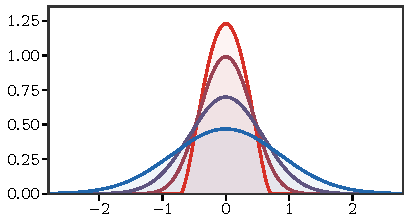
\includegraphics[width=.30\linewidth]{figures/gradflow-heat-versus-porous-medium--heat.pdf} &
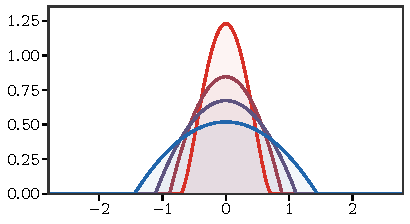
\includegraphics[width=.30\linewidth]{figures/gradflow-heat-versus-porous-medium--porous-medium.pdf} &
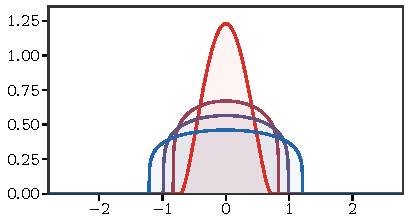
\includegraphics[width=.30\linewidth]{figures/gradflow-heat-versus-porous-medium--porous-medium-m6.pdf}
\end{tabular}
\caption{Entropy-driven Wasserstein gradient flows from the same compact initial density. The heat flow is generated by Shannon entropy $g(\rho)=\rho\log\rho$ and instantly develops Gaussian tails. The porous-medium flows use the power entropy $g(\rho)=\rho^m/(m-1)$, hence $\partial_t\rho=\Delta(\rho^m)$: the middle panel has $m=2$, while the right panel has the stronger nonlinearity $m=6$, i.e. $\partial_t\rho=\Delta(\rho^6)$. Larger powers diffuse mainly where the density is high, producing a flatter core and a sharper compact free boundary.}
\index{Wasserstein!gradient flow}% strictindex
\index{Shannon entropy}% strictindex
\label{fig:gradflow-heat-versus-porous-medium}
\end{figure}

%%%
\paragraph{Interaction Energies.}
\index{energy!interaction}% strictindex

In a similar spirit, to obtain nonlinear evolutions without requiring the measure to have density, one can consider
   \begin{equation}
       f(\alpha) := \iint k(x, y) \d \alpha(x) \d \alpha(y). \label{eq:quadratic-func}
   \end{equation}
   For a symmetric kernel $k$:
   \begin{equation*}
       \delta f(\alpha)(x) = 2 \int k(x, y) \d \alpha(y), \quad \Wgrad f(\alpha)(x) = 2 \int \nabla_x k(x, y) \d \alpha(y).
   \end{equation*}
   For $\alpha_0 = \frac{1}{n} \sum_i \delta_{x_i}$, the flow \eqref{eq:wassflow-pde} implies particles $(x_i(t))_i$ obey:
   \begin{equation*}
       \dot{x}_i(t) = -\frac{2}{n} \sum_j \nabla k(x_i(t), x_j(t)).
   \end{equation*}
	   If $k$ is positive definite, or more generally conditionally positive definite on signed measures of zero total mass as for the energy-distance kernel $k(x,y)=-\norm{x-y}$, and one minimizes the squared kernel discrepancy to a teacher distribution $\beta$, then
\index{teacher distribution}% strictindex
\index{energy distance}% strictindex
\index{signed!measure}% strictindex
   \[
       \norm{\alpha-\beta}_k^2
       =
       \iint k\d\alpha\d\alpha
       -2\int\!\left(\int k(x,y)\d\beta(y)\right)\d\alpha(x)
       +\mathrm{constant}.
       \]
	       Thus MMD-type training energies are exactly an interaction energy plus a linear potential; the teacher distribution appears through the potential $x\mapsto-2\int k(x,y)\d\beta(y)$. The corresponding empirical Wasserstein gradient flow is
\index{teacher distribution}% strictindex
\index{Wasserstein!gradient}% strictindex
\index{gradient!flow}% strictindex
\index{maximum mean discrepancy}% strictindex
\index{Wasserstein!gradient flow}% strictindex
\index{energy!interaction}% strictindex
       \[
		\dot x_i(t)
		=
		-\frac{2}{n}\sum_j\nabla_x k(x_i(t),x_j(t))
		+
		2\int\nabla_x k(x_i(t),y)\d\beta(y).
       \]



	       The first term is a kernelized self-interaction, while the second is the attraction induced by the continuous teacher kernel mean. At the continuum level, characteristic positive-definite kernels, and the Euclidean energy-distance kernel on probability measures, have $\beta$ as the unique minimizer of $\norm{\alpha-\beta}_k^2$. For a finite number of particles, however, the flow can only form a kernelized quadrature of $\beta$, and small particle systems may cover the target modes poorly. Figure~\ref{fig:gradflow-mmd-particle-count} illustrates this finite-particle effect.
\index{kernelized self-interaction}% strictindex
\index{teacher kernel mean}% strictindex
\index{characteristic kernel}% strictindex
\index{kernel!quadrature}% strictindex
\index{probability measure}% strictindex
\index{kernel!positive definite}% strictindex
\index{energy distance}% strictindex

\begin{figure}[ht]
\centering
\begin{tabular}{@{}ccc@{}}
\small $n=10$ particles & \small $n=50$ particles & \small $n=300$ particles \\[-.15em]
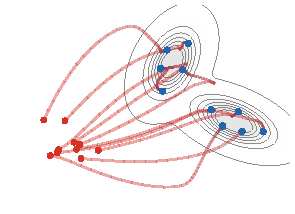
\includegraphics[width=.30\linewidth]{figures/gradflow-mmd-particle-count--n-010.pdf} &
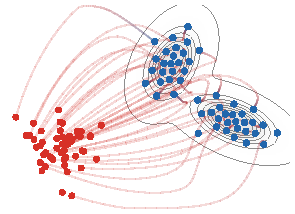
\includegraphics[width=.30\linewidth]{figures/gradflow-mmd-particle-count--n-050.pdf} &
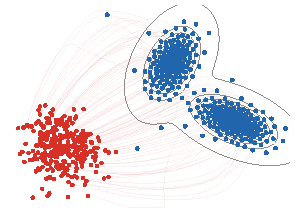
\includegraphics[width=.30\linewidth]{figures/gradflow-mmd-particle-count--n-300.pdf}
\end{tabular}
\caption{Particle count in the deterministic Wasserstein gradient flow of the squared MMD-type discrepancy to a smooth two-Gaussian teacher distribution, using here the energy-distance kernel $k(x,y)=-\norm{x-y}$. The teacher itself is shown only through true density contours, while red dots are a compact shifted Gaussian initialization placed away from the target, red-to-blue curves show a thinned subset of particle trajectories, and blue dots show the stabilized long-time particles. With too few particles, the empirical measure forms a sparse kernelized quadrature and may under-cover the target modes; increasing $n$ makes the particle cloud approximate the continuous target geometry more faithfully.}
\index{teacher distribution}% strictindex
\index{kernel!quadrature}% strictindex
\index{Wasserstein!gradient flow}% strictindex
\index{empirical!measure}% strictindex
\index{energy distance}% strictindex
\label{fig:gradflow-mmd-particle-count}
\end{figure}

The preceding particle flow minimizes a squared kernel discrepancy. Figure~\ref{fig:gradflow-discrepancy-density-comparison} contrasts this with flows generated by three discrepancies toward the same target. For the energy distance and $\Wass_2$, the energy is the unsquared distance, so the Wasserstein velocity is normalized by the current discrepancy value away from the target. The KL case is different: it is a relative-entropy gradient flow and therefore follows the Fokker--Planck diffusion toward the target. The comparison keeps the endpoint fixed and makes the geometry visible through the transient densities.

\begin{figure}[ht]
\centering
\begin{tabular}{@{}ccc@{}}
\small energy distance & \small $\Wass_2$ distance & \small relative entropy \\[-.15em]
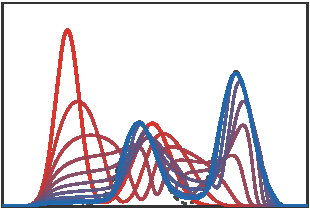
\includegraphics[width=.30\linewidth]{figures/gradflow-discrepancy-density-comparison--energy-distance.pdf} &
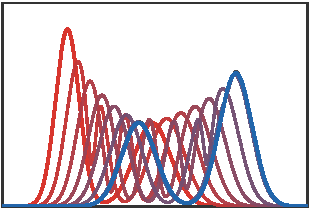
\includegraphics[width=.30\linewidth]{figures/gradflow-discrepancy-density-comparison--w2.pdf} &
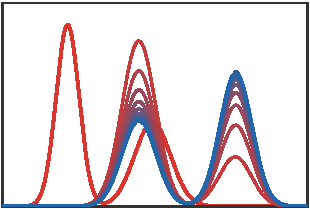
\includegraphics[width=.30\linewidth]{figures/gradflow-discrepancy-density-comparison--kl.pdf}
\end{tabular}
\caption{Wasserstein gradient flows of three discrepancies toward the same one-dimensional Gaussian-mixture target, shown as a dashed black density. The source density is also a Gaussian mixture. Red-to-blue curves are snapshots of $\alpha_t$. The energy-distance and $\Wass_2$ panels descend the unsquared distances and use many equal-weight quantile particles: in one dimension the energy distance is obtained from $\mathrm{ED}^2=2\int |F_{\alpha}-F_{\beta}|^2\d x$, while $\Wass_2$ uses monotone quantile matching. The relative-entropy panel solves the reversible Fokker--Planck equation $\partial_t\rho=\partial_x(\rho_\beta\,\partial_x(\rho/\rho_\beta))$ by an implicit finite-volume scheme, so that $\rho_\beta$ is the discrete stationary density.}
\index{energy distance}% strictindex
\index{relative!entropy}% strictindex
\index{Fokker-Planck equation@Fokker--Planck equation}% strictindex
\index{Wasserstein!gradient flow}% strictindex
\label{fig:gradflow-discrepancy-density-comparison}
\end{figure}

Figure~\ref{fig:gradflow-interaction-particles} complements this target-matching example by isolating three self-interaction regimes.

\begin{figure}[ht]
\centering
\begin{tabular}{@{}ccc@{}}
\small repulsive kernel & \small attractive kernel & \small attraction--repulsion \\[-.15em]
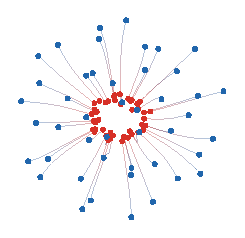
\includegraphics[width=.30\linewidth]{figures/gradflow-interaction-particles--repulsive.pdf} &
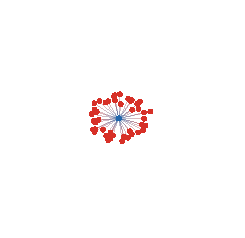
\includegraphics[width=.30\linewidth]{figures/gradflow-interaction-particles--attractive.pdf} &
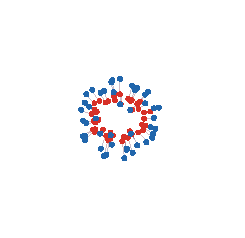
\includegraphics[width=.30\linewidth]{figures/gradflow-interaction-particles--attraction-repulsion.pdf}
\end{tabular}
\caption{Interaction-energy particle flows for three choices of $k$. A positive Gaussian kernel $k(x,y)=\exp(-\norm{x-y}^2/(2\sigma^2))$ produces short-range repulsion under Wasserstein descent; changing its sign produces attraction and collapse; adding a quadratic long-range attraction to the repulsive kernel yields a balanced attraction--repulsion dynamics. The curves use arclength-based red-to-blue coloring along a longer integration of the coupled particle ODE~\eqref{eq:wassflows-particles}.}
\index{particle ODE}% strictindex
\index{energy!interaction}% strictindex
\label{fig:gradflow-interaction-particles}
\end{figure}

Figure~\ref{fig:gradflow-particle-objective-geometries} then compares the trajectory geometries produced by several discrepancies on common source and target clouds.

\begin{figure}[ht]
\centering
\begin{tabular}{@{}cccc@{}}
\small OT rays & \small MMD force & \small Sinkhorn force & \small drifting field \\[-.15em]
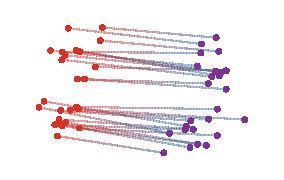
\includegraphics[width=.225\linewidth]{figures/gradflow-particle-objective-geometries--ot-rays.pdf} &
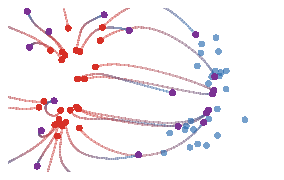
\includegraphics[width=.225\linewidth]{figures/gradflow-particle-objective-geometries--mmd-force.pdf} &
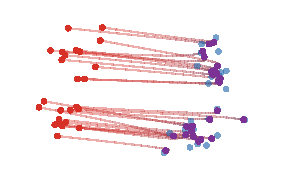
\includegraphics[width=.225\linewidth]{figures/gradflow-particle-objective-geometries--sinkhorn-divergence.pdf} &
\index{Sinkhorn!divergence}% strictindex
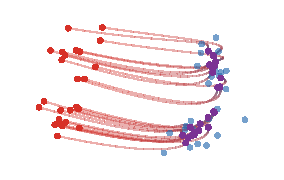
\includegraphics[width=.225\linewidth]{figures/gradflow-particle-objective-geometries--drifting-field.pdf}
\end{tabular}
\caption{Particle trajectories induced by different discrepancy geometries. The red particles and blue target cloud are the same in all panels. Straight OT displacement produces rays from an optimal matching; an MMD-type witness field gives smoother nonlocal forces; the Sinkhorn-divergence force is an entropic, debiased transport attraction; and the normalized drifting field combines attraction to data with self-repulsion. The figure is qualitative: it compares geometric behavior, not solver performance.}
\label{fig:gradflow-particle-objective-geometries}
\end{figure}

\paragraph{Stochastic particles and McKean--Vlasov limits.}
\index{stochastic!particle}% strictindex
\index{McKean-Vlasov limit}% strictindex
\index{McKean-Vlasov equation}% strictindex
More generally, deterministic particle flows have stochastic counterparts, where Brownian noise at the particle level becomes an entropy term at the level of measures. If the drift does not depend on the empirical measure, each particle evolves independently according to
\index{empirical!measure}% strictindex
\[
	\d X_t=b(X_t)\d t+\sqrt{2}\sigma\d B_t,
\]
and the one-particle law $\alpha_t=\rho_t\d x$ directly satisfies the linear Fokker--Planck equation
\index{Fokker-Planck equation@Fokker--Planck equation}% strictindex
\[
	\partial_t\rho_t=-\diverg(b\rho_t)+\sigma^2\Delta\rho_t.
\]

\begin{example}[Langevin drift as a free-energy flow]
	If $b=-\nabla V$, this linear Fokker--Planck equation is the $\Wass_2$ gradient flow of the free energy
	\[
		\rho\mapsto \int V\rho\,\d x+\sigma^2\int\rho\log\rho\,\d x.
	\]
\end{example}

The mean-field case is different: the drift is recomputed from the current empirical distribution of all particles,
\index{empirical!distribution}% strictindex
\index{gradient!flow}% strictindex
\index{mean-field limit}% strictindex
\[
	\d X_i^n(t)=b(X_i^n(t),\al_t^n)\d t+\sqrt{2}\sigma\d B_i(t),
	\qquad
	\al_t^n=\frac1n\sum_{i=1}^n\delta_{X_i^n(t)} .
\]
For finite $n$, the empirical law $\al_t^n$ is itself random. Under suitable Lipschitz, growth and chaotic-initialization assumptions, propagation of chaos states that finitely many particles become asymptotically independent as $n\to\infty$, all with the same deterministic law $\rho_t\d x$; equivalently, the empirical measure $\al_t^n$ converges in probability to this law. The limiting density solves the nonlinear Fokker--Planck, or McKean--Vlasov, equation
\index{Fokker-Planck equation@Fokker--Planck equation}% strictindex
\index{McKean-Vlasov limit}% strictindex
\index{propagation of chaos}% strictindex
\index{empirical!law}% strictindex
\index{McKean-Vlasov equation}% strictindex
\[
	\partial_t \rho_t
	=
	-\diverg\big(b(x,\rho_t)\rho_t\big)
	+
	\sigma^2\Delta\rho_t .
\]
When the interaction drift has variational form
\[
	b(x,\rho)=-\nabla \frac{\delta \mathcal E}{\delta \rho}(x),
\]
	this PDE is the Wasserstein gradient flow of the entropy-regularized energy
\index{Wasserstein!gradient}% strictindex
\index{gradient!flow}% strictindex
\index{Wasserstein!gradient flow}% strictindex
	\[
		\mathcal E(\rho)+\sigma^2\int \rho\log\rho\,\d x .
	\]

For a prescribed target $\beta=\rho_\beta\d x$, take $b=\sigma^2\nabla\log\rho_\beta$. The equivalent Fokker--Planck and score-transport descriptions are
\begin{equation}\label{eq-relative-entropy-three-representations}
	\partial_t\rho_t
	=
	\sigma^2\diverg\!\left(\rho_t\nabla\log\frac{\rho_t}{\rho_\beta}\right),
	\qquad
	v_t=\sigma^2\bigl(\nabla\log\rho_\beta-\nabla\log\rho_t\bigr).
\end{equation}

Figure~\ref{fig:gradflow-fokker-planck-three-representations} compares numerical realizations of precisely these three descriptions.

\begin{figure}[ht]
\centering
\begin{tabular}{@{}c@{}}
\small independent Langevin particles \\[-.15em]
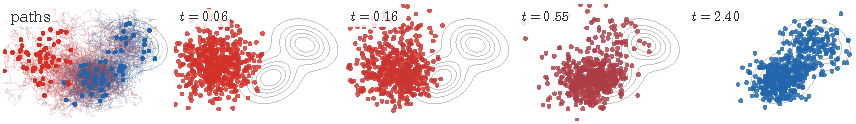
\includegraphics[width=.86\linewidth]{figures/gradflow-fokker-planck-three-representations--langevin-particles.pdf} \\[.25em]
\small deterministic KDE-score particles \\[-.15em]
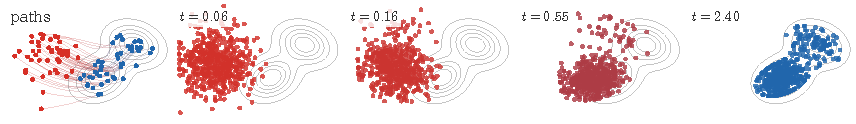
\includegraphics[width=.86\linewidth]{figures/gradflow-fokker-planck-three-representations--kde-particles.pdf} \\[.25em]
\small grid Fokker--Planck density \\[-.15em]
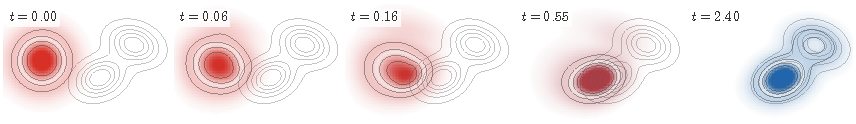
\includegraphics[width=.86\linewidth]{figures/gradflow-fokker-planck-three-representations--grid-pde.pdf}
\end{tabular}
\caption{Three numerical representations of the same entropy-regularized Wasserstein gradient flow of $\KL(\rho|\beta)$, where $\beta$ is a two-Gaussian target shifted to the right of an initially isotropic Gaussian density. The first row simulates independent Langevin particles and displays a thinned set of trajectories in the left panel. The second row evolves many deterministic particles with the score velocity in~\eqref{eq-relative-entropy-three-representations}, estimating $\nabla\log\rho_t$ by a kernel-density estimator; only representative trajectories and particle subsets are displayed. The third row solves the corresponding Fokker--Planck equation on a grid, starting from the initial density in the left panel. The remaining columns use front-loaded times, so that the onset of the flow and the later deformation toward a bimodal law are both visible.}
\index{Wasserstein!gradient flow}% strictindex
\index{Fokker-Planck equation@Fokker--Planck equation}% strictindex
\index{Langevin dynamics}% strictindex
\label{fig:gradflow-fokker-planck-three-representations}
\end{figure}


%%%
\paragraph{Gradient flows under density constraints.}
\index{density!constraint}% strictindex
\index{crowd motion}% strictindex
\index{congestion}% strictindex

The same minimizing-movement formalism also handles nonsmooth energies. A prototypical example is a linear energy, generated by a potential, with a hard upper bound on the density,
\begin{equation}\label{eq-density-constrained-energy}
	f_\kappa(\rho\d x)=\int_\Omega h(x)\rho(x)\d x+
	\iota_{\mathcal K_\kappa}(\rho\d x),
	\qquad
	\mathcal K_\kappa=
	\enscond{\rho\d x\in\Pp_2(\Omega)}{0\leq\rho\leq\kappa\ \text{a.e.}},
\end{equation}
where $\Omega\subset\RR^d$ is a convex domain and $\mathcal K_\kappa$ is assumed nonempty; if $\Omega$ has finite volume, this requires $\kappa|\Omega|\geq1$. The indicator term has no classical first variation; it contributes the normal cone to $\mathcal K_\kappa$ in the Wasserstein first-order condition. The JKO step becomes
\begin{equation}\label{eq-density-constrained-jko}
	\alpha^{k+1}
	\in
	\uargmin{\alpha\in\mathcal K_\kappa}
	\frac{1}{2\tau}\Wass_2^2(\alpha^k,\alpha)+\int_\Omega h\,\d\alpha .
\end{equation}
This is the mathematical mechanism behind macroscopic crowd-motion models with congestion, where the desired velocity $-\nabla h$ is projected onto velocities that do not increase density beyond the maximal value $\kappa$~\cite{maury2010macroscopic,SantambrogioCrowdReview}.
\index{normal cone}% strictindex
\index{maximal density constraint}% strictindex
\index{congestion}% strictindex

The constraint set is compatible with Wasserstein geometry.

\begin{proposition}[Geodesic convexity of density caps]\label{prop-density-cap-geodesic-convex}
\index{density!constraint}% strictindex
\index{convexity!geodesic}% strictindex
	Assume that $\Omega\subset\RR^d$ is convex and let $\kappa>0$. The set $\mathcal K_\kappa$ in~\eqref{eq-density-constrained-energy} is geodesically convex in $\Pp_2(\Omega)$: if $\alpha_0,\alpha_1\in\mathcal K_\kappa$, then the constant-speed $\Wass_2$ geodesic $(\alpha_t)_{t\in[0,1]}$ between them also belongs to $\mathcal K_\kappa$.
\end{proposition}
\begin{proof}
	Assume first that the endpoints have smooth positive densities $\alpha_i=\rho_i\d x$ with $\rho_i\leq\kappa$, and let $T=\nabla\varphi$ be the Brenier map from $\alpha_0$ to $\alpha_1$. Since $\Omega$ is convex, $T_t=(1-t)\Id+tT$ maps $\Omega$ into $\Omega$. The interpolation is $\alpha_t=(T_t)_\sharp\alpha_0$ and
	\[
		\rho_t(T_t(x))=\frac{\rho_0(x)}{\det((1-t)I+t\nabla T(x))}.
	\]
	The concavity of $\det^{1/d}$ on positive semidefinite matrices and the identity $\rho_1(T(x))\det\nabla T(x)=\rho_0(x)$ give
	\[
		\rho_t(T_t(x))^{-1/d}
		\geq
		(1-t)\rho_0(x)^{-1/d}+t\rho_1(T(x))^{-1/d}
		\geq\kappa^{-1/d}.
	\]
	Hence $\rho_t\leq\kappa$ for all $t$. The general case follows by approximation and lower semicontinuity of the $L^\infty$ bound, as in McCann's displacement-convexity theory~\cite{mccann1997convexity}.
\index{Brenier!map}% strictindex
\index{displacement interpolation}% strictindex
\end{proof}

The formal PDE contains a pressure field $p_t$, the Lagrange multiplier of the constraint. With no-flux boundary condition $\rho_t\nabla(h+p_t)\cdot n=0$ on $\partial\Omega$, the constrained gradient flow is the complementarity system
\begin{equation}\label{eq-density-constrained-pressure-flow}
	\partial_t\rho_t=\diverg\left(\rho_t\nabla(h+p_t)\right),
	\qquad
	0\leq\rho_t\leq\kappa,
	\qquad
	p_t\geq0,
	\qquad
	p_t(\kappa-\rho_t)=0.
\end{equation}
The pressure vanishes in the unsaturated region and acts only where $\rho_t=\kappa$, pushing mass away from congested zones so that the density cap remains satisfied.
\index{pressure field}% strictindex
\index{Lagrange multiplier}% strictindex

Figure~\ref{fig:gradflow-density-constrained-flow} shows how decreasing the cap converts free concentration into a saturated region whose width is fixed by mass conservation.

\begin{figure}[H]
\centering
\begin{tabular}{@{}ccc@{}}
\small small cap, $\kappa=.32$ & \small medium cap, $\kappa=.72$ & \small no cap, $\kappa=+\infty$ \\[-.15em]
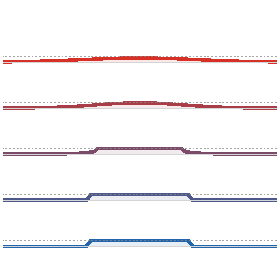
\includegraphics[width=.30\linewidth]{figures/gradflow-density-constrained-flow--kappa-small.pdf} &
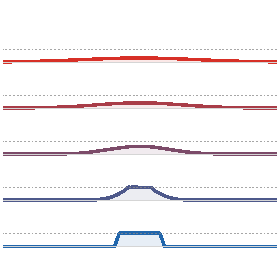
\includegraphics[width=.30\linewidth]{figures/gradflow-density-constrained-flow--kappa-medium.pdf} &
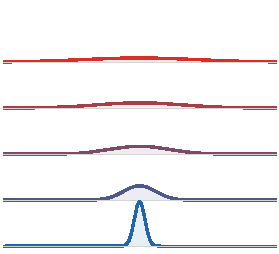
\includegraphics[width=.30\linewidth]{figures/gradflow-density-constrained-flow--unconstrained.pdf}
\end{tabular}
\caption{Density-constrained gradient flow for the attractive quadratic potential $h(x)=\norm{x}^2/2$ in one dimension, computed in quantile variables by explicit Lagrangian descent followed by the isotonic projection enforcing $\partial_s q\geq1/\kappa$. Each panel stacks five times vertically, colored from red to blue, using the same vertical density scale in all three panels. The dashed gray line marks the maximal density $\kappa$ for the constrained runs. A small cap forces the mass to form a wide saturated block, a medium cap allows a narrower congested region, and the unconstrained flow concentrates freely near the minimizer of $h$.}
\index{density!constraint}% strictindex
\index{crowd motion}% strictindex
\index{pressure field}% strictindex
\label{fig:gradflow-density-constrained-flow}
\end{figure}

%%%
\paragraph{Multi-species gradient flows.}
\index{multi-species gradient flow}% strictindex
\index{vector-valued measure}% strictindex
\index{multi-species flow}% strictindex

Several applications involve several densities living on the same physical space: chemical species, color channels, cell populations or competing phases. Let $\Omega\subset\RR^d$ be the physical domain and assume that the component masses $\mathbf m=(m_1,\ldots,m_p)$ are positive and fixed. A convenient notation is
\begin{equation}\label{eq-multispecies-space}
	\Pp_{2,\mathbf m}(\Omega;\RR_+^p)=
	\enscond{\alpha=(\alpha_1,\ldots,\alpha_p)}
	{\alpha_i\in\Mm_+(\Omega),\ \alpha_i(\Omega)=m_i,\ \int_\Omega\norm{x}^2\d\alpha_i(x)<+\infty}.
\end{equation}
Since the components are finite measures rather than necessarily probabilities, set
\begin{equation}\label{eq-multispecies-product-metric}
	\Wass_{2,\oplus}^2(\alpha,\eta)=
	\sum_{i=1}^p m_i\,
	\Wass_2^2\!\left(\frac{\alpha_i}{m_i},\frac{\eta_i}{m_i}\right).
\end{equation}
This is the diagonal, independent-channel geometry; cross-effects may still enter through the energy or through constraints. In the dynamic language used later for vector-valued measures, this is the special case of a diagonal mobility; see Proposition~\ref{prop-diagonal-positive-vector-bb}. The corresponding JKO step is
\begin{equation}\label{eq-multispecies-jko}
	\alpha^{k+1}
	\in
	\uargmin{\alpha\in\Pp_{2,\mathbf m}(\Omega;\RR_+^p)}
		\frac{1}{2\tau}\Wass_{2,\oplus}^2(\alpha^k,\alpha)+f(\alpha).
\end{equation}
For smooth densities and first variations $\phi_i=\delta f/\delta\rho_i$, this yields
\begin{equation}\label{eq-multispecies-pde}
	\partial_t\rho_i=\diverg\left(\rho_i\nabla\phi_i\right),
	\qquad
	\phi_i=\frac{\delta f}{\delta\rho_i},
	\qquad i=1,\ldots,p.
\end{equation}
The equations are independent only if $F$ is separable. Otherwise the coupling enters through the first variations $\phi_i$, not through the metric tensor. Carlier, Chizat and Laborde~\cite{CarlierChizatLabordeDisplacementSmoothness} use displacement smoothness of entropic OT to prove well-posedness of Wasserstein gradient flows that include multi-species systems. Congestion and shared-density variants are closely related to crowd and traffic models~\cite{maury2010macroscopic,CarlierSantambrogioOTCongestion2008,SantambrogioCrowdReview}.
\index{product Wasserstein metric}% strictindex
\index{JKO scheme}% strictindex

A second useful model imposes a pointwise composition constraint. Given a fixed reference density $\beta=b\d x$ with total mass $\sum_i m_i$, set
\begin{equation}\label{eq-multispecies-composition-constraint}
	\mathcal C_\beta=
	\enscond{\alpha\in\Pp_{2,\mathbf m}(\Omega;\RR_+^p)}
	{\sum_{i=1}^p \alpha_i=\beta}.
\end{equation}
The constrained JKO step is
\begin{equation}\label{eq-multispecies-constrained-jko}
	\alpha^{k+1}
	\in
	\uargmin{\alpha\in\mathcal C_\beta}
		\frac{1}{2\tau}\Wass_{2,\oplus}^2(\alpha^k,\alpha)+f(\alpha).
\end{equation}
In the smooth-density regime, the formal constrained flow has a common pressure $\lambda_t$:
\begin{equation}\label{eq-multispecies-constrained-pde}
	\partial_t\rho_i=\diverg\left(\rho_i\nabla(\phi_i-\lambda_t)\right),
	\qquad
	\diverg(b\nabla\lambda_t)=\diverg\left(\sum_{i=1}^p \rho_i\nabla\phi_i\right).
\end{equation}
For the separable Shannon entropy $f(\alpha)=\sum_i\int_\Omega \rho_i\log\rho_i\d x$, this becomes
\begin{equation}\label{eq-multispecies-modified-heat}
	\partial_t\rho_i=\Delta\rho_i-\diverg(\rho_i\nabla\lambda_t),
	\qquad
	\diverg(b\nabla\lambda_t)=\Delta b.
\end{equation}
When $b$ is constant, the pressure can be chosen constant and the system reduces to independent heat equations which nevertheless preserve the pointwise sum $\sum_i\rho_i=b$. This product geometry should be contrasted with the vector-valued Benamou--Brenier distances of Section~\ref{sec-vector-matrix-valued-measures}, where the metric itself can couple the components through a non-diagonal mobility.
\index{Shannon entropy}% strictindex
\index{pressure field}% strictindex
\index{composition constraint}% strictindex

Figure~\ref{fig:gradflow-multispecies-entropy-flow} visualizes this constant-total-density case for two, three, and five species.

\begin{figure}[H]
\centering
\begin{tabular}{@{}ccc@{}}
\small $p=2$ species & \small $p=3$ species & \small $p=5$ species \\[-.15em]
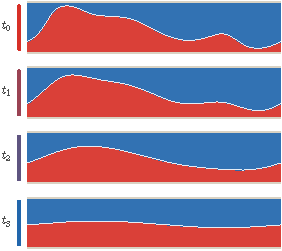
\includegraphics[width=.30\linewidth]{figures/gradflow-multispecies-entropy-flow--two-species.pdf} &
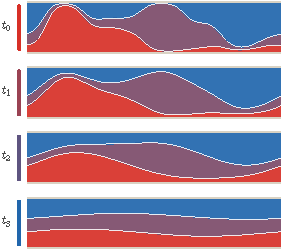
\includegraphics[width=.30\linewidth]{figures/gradflow-multispecies-entropy-flow--three-species.pdf} &
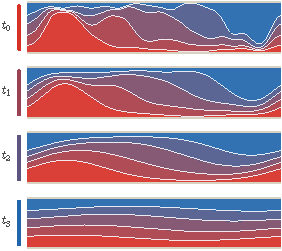
\includegraphics[width=.30\linewidth]{figures/gradflow-multispecies-entropy-flow--five-species.pdf}
\end{tabular}
\caption{Multi-species entropy flow under the shared-density constraint $\sum_i\rho_i=1$ on the periodic interval. Each row is a time snapshot of the stacked densities, with the species shown as colored bands and time increasing from top to bottom. For a constant total density, the pressure in~\eqref{eq-multispecies-modified-heat} is constant, so each component follows the heat equation while the sum of the bands remains exactly flat.}
\index{multi-species gradient flow}% strictindex
\index{Shannon entropy}% strictindex
\index{density!constraint}% strictindex
\label{fig:gradflow-multispecies-entropy-flow}
\end{figure}

\section{Unbalanced Wasserstein--Fisher--Rao Gradient Flows}
\label{sec-dynamic-unbalanced-wfr-flows}
\index{unbalanced!gradient flow}% strictindex
\index{Wasserstein-Fisher-Rao@Wasserstein--Fisher--Rao}% strictindex
\index{birth-death dynamics}% strictindex
\index{Wasserstein-Fisher-Rao distance}% strictindex

The Wasserstein gradient flows above conserve total mass, because their tangent vectors are generated by continuity equations. When the unknown measure represents an intensity, a population or a cloud of trainable particles, it is often useful to combine spatial motion with creation and destruction of mass. The dynamic unbalanced distance defined in Section~\ref{sec-unbalanced-ot}, through the balance-equation formula~\eqref{eq-dynamic-unbalanced-ot}, gives exactly this geometry.

\begin{defn}[WFR minimizing movement]\label{def-wfr-jko-gradient-flow}
\index{JKO scheme}% strictindex
	Let $f:\Mm_+(\RR^d)\to\RR\cup\{+\infty\}$ be an energy on positive finite measures and let $\WFR_\kappa$ be the Wasserstein--Fisher--Rao distance with growth scale $\kappa>0$, defined by the dynamic balance-equation formulation~\eqref{eq-dynamic-unbalanced-ot} and its static equivalence in Proposition~\ref{prop-static-dynamic-unbalanced}. The unbalanced JKO step is
	\begin{equation}\label{eq-wfr-jko}
		\alpha^{k+1}
		\in
		\uargmin{\alpha\in\Mm_+(\RR^d)}
		\frac{1}{2\tau}\WFR_\kappa^2(\alpha^k,\alpha)+f(\alpha).
	\end{equation}
	The continuous-time limit, when it exists, is called the $\WFR_\kappa$ gradient flow of $f$.
\end{defn}

Formally, a smooth curve $\alpha_t=\rho_t\d x$ has tangent vectors of the form
\[
	\partial_t\rho_t+\diverg(\rho_t v_t)=g_t\rho_t,
\]
with squared norm $\int(\norm{v_t}^2+\kappa^2 g_t^2)\rho_t\d x$. This is the infinitesimal version of the balance-equation action in Chapter~\ref{sec-dynamic-optimal-transport}.

\begin{proposition}[Formal WFR gradient-flow PDE]\label{prop-wfr-gradient-flow-pde}
\index{Wasserstein-Fisher-Rao@Wasserstein--Fisher--Rao}% strictindex
\index{balance equation}% strictindex
	Assume that $f$ has a smooth first variation $\phi_t=\delta f(\alpha_t)$ and that $\alpha_t=\rho_t\d x$ is smooth and positive. The formal $\WFR_\kappa$ gradient flow of $f$ is
\index{Wasserstein-Fisher-Rao distance}% strictindex
	\begin{equation}\label{eq-wfr-gradient-flow-pde}
		\partial_t\rho_t
		=
		\diverg(\rho_t\nabla\phi_t)
		-
		\frac{1}{\kappa^2}\phi_t\rho_t .
	\end{equation}
	Along such a smooth solution,
	\begin{equation}\label{eq-wfr-energy-dissipation}
		\frac{\d}{\d t}f(\alpha_t)
		=
		-\int
		\left(\norm{\nabla\phi_t}^2+\frac{1}{\kappa^2}\phi_t^2\right)\rho_t\,\d x
		\leq 0 .
	\end{equation}
\end{proposition}
\begin{proof}
	For an infinitesimal tangent pair $(v,g)$, the density variation is $\zeta=-\diverg(\rho v)+g\rho$. The first variation of $f$ is
	\[
		\int \phi\,\zeta
		=
		\int \dotp{\nabla\phi}{v}\rho\,\d x+\int \phi g\rho\,\d x,
	\]
	after integration by parts. For the inner product
	\[
		\dotp{(v,g)}{(\tilde v,\tilde g)}_\rho
		=
		\int \dotp{v}{\tilde v}\rho\,\d x+\kappa^2\int g\tilde g\rho\,\d x,
	\]
	the Riesz representative is $(\nabla\phi,\phi/\kappa^2)$. Steepest descent therefore uses $(v,g)=(-\nabla\phi,-\phi/\kappa^2)$, which gives~\eqref{eq-wfr-gradient-flow-pde}.
	Substituting this pair in the first-variation formula gives
	\[
		\frac{\d}{\d t}f(\alpha_t)
		=
		-\int
		\left(\norm{\nabla\phi_t}^2+\frac{1}{\kappa^2}\phi_t^2\right)\rho_t\,\d x,
	\]
	which is~\eqref{eq-wfr-energy-dissipation}.
\end{proof}

The reaction term makes additive constants in the first variation meaningful: adding a constant to $\phi$ changes the global growth rate. This is not a defect but the infinitesimal signature of optimizing over positive finite measures, rather than on the probability simplex. The rigorous metric-space construction of Kantorovich--Fisher--Rao and WFR gradient flows is developed in~\cite{gallouet2017jko,2017-chizat-focm,2015-chizat-unbalanced}. Chizat's measure-optimization framework relates weight-changing gradient methods to mirror- and Bregman-type descents on positive measures~\cite{Chizat2019SparseOptimization,Chizat2021GradientMethodsMeasures}. In machine learning, birth--death dynamics use the same reaction intuition to let a particle population reweight, remove and create neurons during training~\cite{Rotskoff2019BirthDeath}.

\begin{example}[Relative entropy and birth--death relaxation]\label{ex-wfr-kl-flow}
\index{relative!entropy}% strictindex
\index{Fokker-Planck equation@Fokker--Planck equation}% strictindex
	Let $\beta=b\d x$ and use the finite-measure relative entropy
	\[
		f(\alpha)=\KL(\alpha|\beta)
		=
		\int
		\left(\rho\log\frac{\rho}{b}-\rho+b\right)\d x,
		\qquad
		\alpha=\rho\d x.
	\]
	This is the Csisz{\'a}r divergence on positive measures; it is nonnegative and is minimized, without imposing a mass constraint, at $\alpha=\beta$. Its first variation is $\delta f(\alpha)=\log(\rho/b)$. The balanced $\Wass_2$ flow, when the total mass is fixed, is the Fokker--Planck equation
\index{Fokker-Planck equation@Fokker--Planck equation}% strictindex
	\[
		\partial_t\rho_t
		=
		\diverg\left(\rho_t\nabla\log\frac{\rho_t}{b}\right)
		=
		\Delta\rho_t-\diverg(\rho_t\nabla\log b),
	\]
	whereas the $\WFR_\kappa$ flow is
	\begin{equation}\label{eq-wfr-kl-flow}
		\partial_t\rho_t
		=
		\Delta\rho_t-\diverg(\rho_t\nabla\log b)
		-
		\frac{1}{\kappa^2}\rho_t\log\frac{\rho_t}{b}.
	\end{equation}
	The first two terms transport and diffuse mass, while the last term kills mass where $\rho_t>b$ and creates it where $\rho_t<b$.
\end{example}

Figure~\ref{fig:gradflow-wfr-unbalanced-flow} contrasts this reaction-assisted relaxation with its mass-preserving Wasserstein counterpart.

\begin{figure}[ht]
\centering
\begin{tabular}{@{}cc@{}}
\small balanced $\Wass_2$ flow & \small unbalanced $\WFR_\kappa$ flow \\[-.15em]
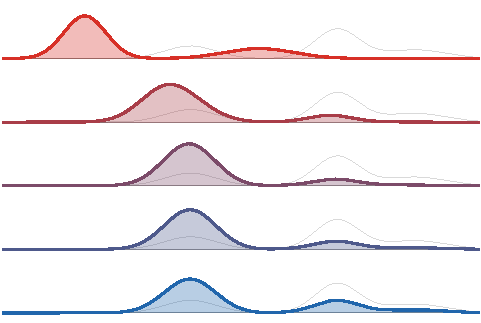
\includegraphics[width=.46\linewidth]{figures/gradflow-wfr-unbalanced-flow--balanced.pdf} &
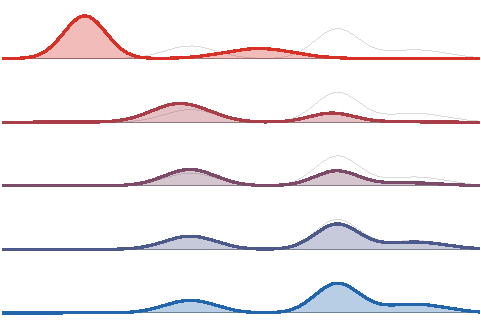
\includegraphics[width=.46\linewidth]{figures/gradflow-wfr-unbalanced-flow--unbalanced.pdf}
\end{tabular}
\caption{Balanced and unbalanced gradient flows of $\KL(\rho|\beta)$ for one-dimensional Gaussian mixtures. In each panel the colored density stacks correspond to five increasing times, from red to blue, and the faint gray curve repeated on each row is the target mixture $\beta$. The balanced Wasserstein flow is the conservative Fokker--Planck equation, so mass must move through the low-density region between modes. The $\WFR_\kappa$ flow adds the birth--death reaction term in~\eqref{eq-wfr-kl-flow}; it attenuates overrepresented regions and creates missing mass near target modes, reaching the target shape much faster.}
\index{Wasserstein!gradient flow}% strictindex
\index{Wasserstein-Fisher-Rao@Wasserstein--Fisher--Rao}% strictindex
\index{birth-death dynamics}% strictindex
\index{Fokker-Planck equation@Fokker--Planck equation}% strictindex
\label{fig:gradflow-wfr-unbalanced-flow}
\end{figure}

\section{Geodesic Convexity and Convergence}
\index{convexity!geodesic}% strictindex
\label{sec-geodesic-convexity}

Geodesic convexity is the convexity notion adapted to Wasserstein geometry. It is the condition that turns the formal gradient-flow calculus into a convergence theory.
\index{gradient!flow}% strictindex
\index{geodesic!convexity}% strictindex

\paragraph{Geodesics and convexity.}

A constant-speed $\Wass_2$ geodesic between $\alpha_0$ and $\alpha_1$ is obtained, as in Definition~\ref{def-w2-geodesic-induced-by-plan}, from any optimal coupling $\pi^\star\in\Couplings(\alpha_0,\alpha_1)$ by the McCann interpolation
\index{optimal coupling}% strictindex
\index{constant-speed geodesic}% strictindex
\index{McCann interpolation}% strictindex
\[
	\alpha_t=((1-t)P_0+tP_1)_\sharp\pi^\star,
	\qquad t\in[0,1],
\]
where $P_0(x,y)=x$ and $P_1(x,y)=y$. If the optimal plan is induced by a Brenier map $T$, this reduces to $((1-t)\Id+tT)_\sharp\alpha_0$. The coupling formula is important because geodesics exist even when no Monge map exists, for instance when a Dirac mass must split.
\index{Monge!problem}% strictindex
\index{optimal plan}% strictindex
\index{Brenier!map}% strictindex
\index{Dirac mass}% strictindex

\begin{defn}[Geodesic convexity]\label{def-geodesic-convexity}
\index{convexity!geodesic}% strictindex
	A functional $f$ on $\Pp_2(\RR^d)$ is geodesically convex if for every $\Wass_2$ geodesic $(\alpha_t)_t$,
	\[
		f(\alpha_t)\leq (1-t)f(\alpha_0)+t f(\alpha_1).
	\]
	It is $\lambda$-geodesically convex if the right-hand side is improved by $-\frac{\lambda}{2}t(1-t)\Wass_2^2(\alpha_0,\alpha_1)$.
\end{defn}

\begin{prop}[Basic geodesically convex energies]\label{prop-basic-geodesic-convexity}
\index{convexity!geodesic}% strictindex
	The following formal statements hold on $\Pp_2(\RR^d)$.
	\begin{enumerate}
		\item If $h$ is convex, then $\alpha\mapsto\int h\d\alpha$ is geodesically convex; if $h$ is $\lambda$-strongly convex, it is $\lambda$-geodesically convex.
		\item If $W(x-y)$ is convex as a function of the displacement, then $\alpha\mapsto\frac12\iint W(x-y)\d\alpha(x)\d\alpha(y)$ is geodesically convex.
		\item Shannon entropy $\alpha\mapsto\int\rho\log\rho\,\d x$ is geodesically convex.
\index{Shannon entropy}% strictindex
		\item The relative entropy $\KL(\alpha|\gamma)$ with $\d\gamma=e^{-V}\d x/Z$ is $\lambda$-geodesically convex when $V$ is $\lambda$-strongly convex.
\index{relative!entropy}% strictindex
	\end{enumerate}
\end{prop}
\begin{proof}
	Along a Monge geodesic $X_t=(1-t)X_0+tX_1$, convexity of $h$ gives $h(X_t)\leq(1-t)h(X_0)+t h(X_1)$, and strong convexity gives the additional quadratic term; integrating proves the first claim. The interaction claim follows similarly by applying convexity of $W$ to pairwise differences $X_t-X_t'=(1-t)(X_0-X_0')+t(X_1-X_1')$ and integrating over two independent copies. The entropy claim is McCann's displacement convexity theorem; at the density level it follows from the concavity of the Jacobian determinant under the interpolation of optimal maps. Finally, $\KL(\alpha|\gamma)=\int\rho\log\rho\,\d x+\int V\d\alpha+\mathrm{constant}$, so it is the sum of displacement-convex entropy and a $\lambda$-geodesically convex linear potential.
\index{displacement convexity}% strictindex
\index{Jacobian determinant}% strictindex
\index{convexity!geodesic}% strictindex
\index{Monge!geodesic}% strictindex
\end{proof}

\begin{example}[Squared Wasserstein distance need not be geodesically convex]

The squared distance to a fixed measure is not geodesically convex in general. This is a sharp contrast with Hilbert spaces, where \(x\mapsto\norm{x-y}^2\) is convex along line segments. In \(\Pp_2(\RR^d)\), \(d\geq2\), take
\[
	\beta=\frac12\de_{(-1/2,-1/2)}+\frac12\de_{(1/2,1/2)},
	\quad
	\alpha_0=\frac12\de_{(-1,0)}+\frac12\de_{(1,0)},
	\quad
	\alpha_1=\frac12\de_{(0,-1)}+\frac12\de_{(0,1)} .
\]
One optimal coupling between \(\alpha_0\) and \(\alpha_1\) matches \((-1,0)\) with \((0,1)\) and \((1,0)\) with \((0,-1)\). The associated geodesic has midpoint
\[
	\alpha_{1/2}=\frac12\de_{(-1/2,1/2)}+\frac12\de_{(1/2,-1/2)} .
\]
Then
\[
	\Wass_2^2(\alpha_0,\beta)
	=
	\Wass_2^2(\alpha_1,\beta)
	=
	\frac12,
	\qquad
	\Wass_2^2(\alpha_{1/2},\beta)
	=
	1,
\]
which violates geodesic convexity. Thus objectives built from squared Wasserstein distances can be non-convex in the Wasserstein geometry itself. This is one reason why optimal quantization, which minimizes \(\Wass_2^2(\alpha,\nu)\) over \(m\)-atomic measures \(\nu\), leads to non-convex algorithms such as Lloyd's method; see Section~\ref{sec-optimal-quantization} and Algorithm~\ref{alg:lloyd-quantization}.
\index{Wasserstein!squared distance}% strictindex
\index{quantization!optimal}% strictindex
\index{Lloyd!algorithm}% strictindex
\end{example}

\begin{rem}[Target discrepancies are usually semiconcave]\label{rem-target-discrepancies-semiconcave}
\index{geodesic!semiconcavity}% strictindex
\index{generative model}% strictindex
	The preceding example is a useful warning. Losses of the form
	\(\alpha\mapsto D(\alpha,\beta)\), where \(\beta\) is a fixed target
	distribution, are rarely geodesically convex in the transport geometry. This is unfortunate for generative AI and generative modeling more broadly: training a distribution to match data by decreasing \(\Wass_2^2(\alpha,\beta)\), \(\SW_2^2(\alpha,\beta)\), or similar discrepancies should not be expected to inherit the convex behavior of Euclidean least squares.

	The squared Wasserstein loss has the opposite one-sided curvature: it is \(2\)-geodesically semiconcave along \(\Wass_2\) geodesics. More precisely, if \((\alpha_t)_{t\in[0,1]}\) is a constant-speed \(\Wass_2\) geodesic, then
	\[
		\Wass_2^2(\alpha_t,\beta)
		\geq
		(1-t)\Wass_2^2(\alpha_0,\beta)
		+
		t\Wass_2^2(\alpha_1,\beta)
		-
		t(1-t)\Wass_2^2(\alpha_0,\alpha_1).
	\]
	This is the standard \(2\)-geodesic semiconcavity convention for squared distances, often informally called ``\(2\)-concavity'': the graph may fall below the chord, but only by the quadratic correction \(t(1-t)\Wass_2^2(\alpha_0,\alpha_1)\). Equivalently, \(-\Wass_2^2(\cdot,\beta)\) is \((-2)\)-geodesically convex in the convention of Definition~\ref{def-geodesic-convexity}.

	To prove the estimate, write
	\(\alpha_t=((1-t)P_0+tP_1)_\sharp\pi_{01}\), where \(\pi_{01}\) is optimal between \(\alpha_0\) and \(\alpha_1\). Fix \(t\), put \(Z=(1-t)X_0+tX_1\), take an optimal coupling between \(\alpha_t\) and \(\beta\), and glue it with a disintegration of \(\pi_{01}\) over \(Z\). This gives random variables \((X_0,X_1,Y)\) such that \((Z,Y)\) is optimal between \(\alpha_t\) and \(\beta\), while \((X_0,X_1)\) is optimal between \(\alpha_0\) and \(\alpha_1\). Since \((X_i,Y)\) are admissible couplings between \(\alpha_i\) and \(\beta\),
	\[
		\Wass_2^2(\alpha_i,\beta)\leq \EE\norm{X_i-Y}^2,
		\qquad i=0,1.
	\]
	The Euclidean identity
	\[
		(1-t)\norm{X_0-Y}^2+t\norm{X_1-Y}^2
		=
		\norm{Z-Y}^2+t(1-t)\norm{X_0-X_1}^2
	\]
	then gives the claim after taking expectations.

	The sliced loss has the same flavor, but one must keep track of which geometry is used. The projection of a \(\Wass_2\) geodesic need not be the monotone one-dimensional geodesic between the projected endpoint measures. Fix a direction $\theta$ and project $\pi_{01}$ onto $(\dotp{\theta}{X_0},\dotp{\theta}{X_1})$. This coupling generates the projected curve but need not be optimal. At time $t$, couple the projected $\alpha_t$ optimally to the projected $\beta$, then glue over the projected interpolated variable. The Euclidean identity applies with correction cost $\EE|\dotp{\theta}{X_0-X_1}|^2$. Integrating with the normalization of Definition~\ref{def-sliced-wasserstein} gives, along the original \(\Wass_2\) geodesic,
	\[
		\SW_2^2(\alpha_t,\beta)
		\geq
		(1-t)\SW_2^2(\alpha_0,\beta)
		+
		t\SW_2^2(\alpha_1,\beta)
		-
		\frac{t(1-t)}{d}\Wass_2^2(\alpha_0,\alpha_1),
	\]
	because the projection cost satisfies
	\(\int_{\Sphere^{d-1}}\abs{\dotp{\theta}{x_0-x_1}}^2\d\sigma(\theta)=\norm{x_0-x_1}^2/d\) and \(\pi_{01}\) is \(\Wass_2\)-optimal. Thus this is a semiconcavity estimate for the sliced discrepancy along \(\Wass_2\) geodesics, with a \(\Wass_2\)-controlled correction. If one instead works in the idealized Hilbert embedding by projected quantile functions, straight sliced chords satisfy the exact identity with the last term \(\SW_2^2(\alpha_0,\alpha_1)\). The caveat, discussed in the paragraph on intrinsic sliced length in Section~\ref{sec-sliced-wasserstein}, is that such straight chords need not be realized by actual measures on \(\RR^d\).
\end{rem}

\paragraph{Convergence of the flow.}

In general, analyzing \eqref{eq:wassflow-pde} is delicate. The cleanest case is when $f$ is geodesically convex in the sense above. This condition is the Wasserstein analogue of convexity in Euclidean gradient descent.

\begin{prop}[Energy decay for convex Wasserstein flows]\label{prop-convex-wass-flow-rate}
\index{energy!decay}% strictindex
\index{Wasserstein!flow}% strictindex
	Assume formally that $f$ is geodesically convex, admits a smooth first variation, and has a minimizer $\alpha^\star$. Let $(\alpha_t)_t$ be a smooth solution of the Wasserstein gradient flow
\index{first variation}% strictindex
\index{Wasserstein!gradient}% strictindex
\index{gradient!flow}% strictindex
\index{Wasserstein!gradient flow}% strictindex
	\[
		\partial_t\alpha_t+\diverg(\alpha_t v_t)=0,
		\qquad
		v_t=-\Wgrad f(\alpha_t).
	\]
	Then
	\[
		\frac{\d}{\d t} f(\alpha_t)
		=
		-\int \norm{\Wgrad f(\alpha_t)(x)}^2\,\d\alpha_t(x)
		\leq 0.
	\]
	If $T_t$ is the optimal map from $\alpha_t$ to $\alpha^\star$, then
	\[
		f(\alpha_t)-f(\alpha^\star)
		\leq
		-\frac{\d}{\d t}\frac12 \Wass_2^2(\alpha_t,\alpha^\star),
	\]
	and consequently
	\[
		f(\alpha_t)-f(\alpha^\star)
		\leq
		\frac{\Wass_2^2(\alpha_0,\alpha^\star)}{2t}.
	\]
	If $f$ is $\lambda$-geodesically convex with $\lambda>0$, then
	\[
		f(\alpha_t)-f(\alpha^\star)
		\leq
		e^{-2\lambda t}\bigl(f(\alpha_0)-f(\alpha^\star)\bigr).
	\]
\end{prop}

\begin{proof}
	The chain rule and Proposition~\ref{prop-formal-wass-gradient} give
	\[
		\frac{\d}{\d t}f(\alpha_t)
		=
		\int \dotp{\Wgrad f(\alpha_t)(x)}{v_t(x)}\,\d\alpha_t(x)
		=
		-\int \norm{\Wgrad f(\alpha_t)(x)}^2\,\d\alpha_t(x).
	\]
	Geodesic convexity along the geodesic
\index{convexity!geodesic}% strictindex
\index{geodesic!convexity}% strictindex
	$((1-s)\Id+sT_t)_\sharp\alpha_t$ gives
	\[
		f(\alpha^\star)-f(\alpha_t)
		\geq
		\int \dotp{\Wgrad f(\alpha_t)(x)}{T_t(x)-x}\,\d\alpha_t(x).
	\]
	Since $v_t=-\Wgrad f(\alpha_t)$, this reads
	\[
		f(\alpha_t)-f(\alpha^\star)
		\leq
		\int \dotp{v_t(x)}{T_t(x)-x}\,\d\alpha_t(x).
	\]
	The standard first-variation formula for the squared Wasserstein distance gives
\index{Wasserstein!distance}% strictindex
	\[
		\frac{\d}{\d t}\frac12\Wass_2^2(\alpha_t,\alpha^\star)
		=
		\int \dotp{x-T_t(x)}{v_t(x)}\,\d\alpha_t(x),
	\]
	which proves the differential inequality. Integrating it from $0$ to $t$ and using the monotonicity of $s\mapsto f(\alpha_s)$ gives
	\[
		t\bigl(f(\alpha_t)-f(\alpha^\star)\bigr)
		\leq
		\int_0^t \bigl(f(\alpha_s)-f(\alpha^\star)\bigr)\,\d s
		\leq
		\frac12\Wass_2^2(\alpha_0,\alpha^\star).
	\]
	If $f$ is $\lambda$-geodesically convex, the Wasserstein analogue of strong convexity gives the slope inequality
	\[
		\int\norm{\Wgrad f(\alpha_t)}^2\d\alpha_t
		\geq
		2\lambda\bigl(f(\alpha_t)-f(\alpha^\star)\bigr).
	\]
	Combining it with the energy dissipation identity yields
\index{energy!dissipation}% strictindex
	\[
		\frac{\d}{\d t}\bigl(f(\alpha_t)-f(\alpha^\star)\bigr)
		\leq
		-2\lambda\bigl(f(\alpha_t)-f(\alpha^\star)\bigr),
	\]
	and Gronwall's lemma gives the exponential rate.
\end{proof}

\begin{prop}[Convex examples covered by the theory]\label{prop-convex-flow-examples}
	The hypotheses of Proposition~\ref{prop-convex-wass-flow-rate} are satisfied in the following standard cases, at least at the formal smooth level used in this section.
	\begin{enumerate}
		\item For the linear energy $f(\alpha)=\int h\d\alpha$, geodesic convexity holds when $h$ is convex. If $h$ is $\lambda$-strongly convex, then $f$ is $\lambda$-geodesically convex and the flow enjoys the exponential rate of Proposition~\ref{prop-convex-wass-flow-rate}.
\index{convexity!geodesic}% strictindex
		\item For the interaction energy $f(\alpha)=\frac12\iint W(x-y)\d\alpha(x)\d\alpha(y)$, geodesic convexity holds when $W$ is convex and even. This covers repulsive or attractive pairwise models whose displacement cost has no non-convex wells.
\index{energy!interaction}% strictindex
		\item The Shannon entropy $f(\alpha)=\int\rho\log\rho\,\d x$ and, more generally, McCann displacement-convex internal energies generate diffusion-type Wasserstein gradient flows.
\index{Wasserstein!gradient}% strictindex
\index{gradient!flow}% strictindex
\index{Wasserstein!gradient flow}% strictindex
\index{Shannon entropy}% strictindex
		\item If $\gamma=Z^{-1}e^{-V}\d x$ and $V$ is $\lambda$-strongly convex, then the relative entropy $\KL(\alpha|\gamma)$ is $\lambda$-geodesically convex. Its flow is the Fokker--Planck equation with invariant law $\gamma$.
\index{Fokker-Planck equation@Fokker--Planck equation}% strictindex
\index{relative!entropy}% strictindex
	\end{enumerate}
\end{prop}
\begin{proof}
	Let $(\alpha_t)_t$ be the McCann interpolation between $\alpha_0$ and $\alpha_1$, written with an optimal coupling as $X_t=(1-t)X_0+tX_1$. For a linear energy, Jensen's inequality gives
\index{Jensen inequality}% strictindex
\index{optimal coupling}% strictindex
\index{McCann interpolation}% strictindex
	\[
		h(X_t)\leq(1-t)h(X_0)+t h(X_1),
	\]
	and the strong convexity version gives the additional term $-\frac{\lambda}{2}t(1-t)\norm{X_0-X_1}^2$. Integrating over the optimal coupling proves geodesic convexity and $\lambda$-geodesic convexity.
\index{convexity!geodesic}% strictindex

	For interaction energies, use two independent copies of the optimal coupling. The pairwise displacement evolves as
\index{optimal coupling}% strictindex
\index{energy!interaction}% strictindex
	\[
		X_t-X_t'=(1-t)(X_0-X_0')+t(X_1-X_1').
	\]
	Convexity of $W$ gives the convexity inequality after integration over the product coupling. Evenness of $W$ ensures that the interaction is symmetric in the two particles and matches the usual factor $1/2$ in~\eqref{eq:quadratic-func}.
\index{product!coupling}% strictindex

	The entropy claim is McCann's displacement-convexity theorem. For smooth positive densities and Brenier maps, it follows from the change-of-variables formula and the concavity of the determinant along positive matrices; the general statement is obtained by approximation. Finally,
\index{change of variables formula}% strictindex
\index{displacement convexity}% strictindex
\index{Brenier!map}% strictindex
	\[
		\KL(\alpha|\gamma)=\int\rho\log\rho\,\d x+\int V\d\alpha+\log Z,
	\]
	so it is the sum of the displacement-convex entropy and the $\lambda$-geodesically convex linear potential generated by $V$. Proposition~\ref{prop-convex-wass-flow-rate} then applies to all four cases.
\end{proof}

The interaction criterion above asks for convexity of the kernel on the whole ambient space. In one dimension there is a sharper self-interaction mechanism: along Wasserstein geodesics, quantiles remain ordered, so distances between two ordered copies of the same moving measure evolve by convex combinations inside $\RR_+$. This is the quantile form of one-dimensional displacement convexity discussed in standard references such as~\cite{SantambrogioBook}, and it explains why the negative-distance kernel can behave better in one dimension than its non-convex ambient formula suggests~\cite{DuongRuxSteinSteidl2024DistanceMMD}.
\index{quantile!function}% strictindex
\index{energy!interaction}% strictindex
\index{energy distance}% strictindex

\begin{prop}[One-dimensional self-interaction kernels]\label{prop-1d-interaction-halfline-convex}
\index{one-dimensional!transport}% strictindex
\index{convexity!geodesic}% strictindex
	Let $\varphi:\RR_+\to\RR$ be convex and assume that the following integrals are finite. On $\Pp_2(\RR)$, define
	\[
		\mathcal I_\varphi(\alpha)
		\eqdef
		\frac12\iint \varphi(|x-y|)\d\alpha(x)\d\alpha(y).
	\]
	Then $\mathcal I_\varphi$ is geodesically convex for $\Wass_2$ on $\Pp_2(\RR)$. In particular, the choice $\varphi(r)=-r$ is admissible, even though $z\mapsto-|z|$ is not convex on $\RR$.

	Fix also $\beta\in\Pp_2(\RR)$. For the conditionally positive definite kernel $k(x,y)=-|x-y|$, the squared MMD of Definition~\ref{def-kernel-mmd-norm}, equivalently the squared energy distance,
	\[
		\mathcal E_\beta(\alpha)
		\eqdef
		\MMD_k^2(\alpha,\beta)
		=
		\iint -|x-y|\,\d(\alpha-\beta)(x)\d(\alpha-\beta)(y),
	\]
	is geodesically convex as a function of $\alpha$.
\end{prop}
\begin{proof}
	Let $Q_0,Q_1$ be the quantile functions of $\alpha_0,\alpha_1$, and let $Q_t=(1-t)Q_0+tQ_1$ be the quantile function of the one-dimensional $\Wass_2$ geodesic $\alpha_t$. For $r>s$, monotonicity gives $Q_i(r)-Q_i(s)\geq0$ for $i=0,1$, and hence
	\[
		Q_t(r)-Q_t(s)
		=
		(1-t)(Q_0(r)-Q_0(s))+t(Q_1(r)-Q_1(s)).
	\]
	Using the symmetry of the double integral and ignoring the diagonal, one can write
	\[
		\mathcal I_\varphi(\alpha_t)
		=
		\int_0^1\int_0^r
		\varphi(Q_t(r)-Q_t(s))\,\d s\,\d r.
	\]
	Convexity of $\varphi$ on $\RR_+$ gives the desired convexity after integration. For $\varphi(r)=-r$, the inequality is an equality because $\varphi$ is affine on $\RR_+$.

	For the energy distance, write $Q_\beta$ for the quantile function of $\beta$ and express the functional in quantile variables:
	\[
		\mathcal E_\beta(\alpha)
		=
		2\int_0^1\!\!\int_0^1 |Q_\alpha(r)-Q_\beta(s)|\,\d r\,\d s
		-
		\int_0^1\!\!\int_0^1 |Q_\alpha(r)-Q_\alpha(s)|\,\d r\,\d s
		+\mathrm{constant}.
	\]
	The positive cross-distance term is convex in $Q_\alpha$, since the absolute value is convex and $Q_t$ is affine in $t$. The self-distance term is affine along quantile geodesics because
	\[
		\int_0^1\!\!\int_0^1 |Q_t(r)-Q_t(s)|\,\d r\,\d s
		=
		2\int_0^1\int_0^r (Q_t(r)-Q_t(s))\,\d s\,\d r.
	\]
	Thus $\alpha\mapsto\mathcal E_\beta(\alpha)$ is geodesically convex.
\index{maximum mean discrepancy}% strictindex
\index{energy distance}% strictindex
\end{proof}

The last statement should be read for the full energy-distance combination. The raw attractive term $\alpha\mapsto-\iint |x-y|\,\d\alpha(x)\d\beta(y)$ alone is concave in quantile variables; convexity comes from the MMD combination, namely a positive cross-distance term minus an affine self-distance term.

\paragraph{Convexity and curvature.}

The same language is not restricted to subsets of $\RR^d$. If $(\X,\dist,\mathfrak m)$ is a geodesic metric-measure space, $\Wass_2$ geodesics can be defined by transporting each pair of endpoints along metric geodesics, or more intrinsically by dynamical optimal plans on path space, as discussed in Section~\ref{sec-kantorovich-plan-interpolation}. Given a reference measure $\mathfrak m$, the entropy relative to $\mathfrak m$ is
\index{metric-measure space}% strictindex
\index{geodesic!space}% strictindex
\index{relative!entropy}% strictindex
\index{dynamical optimal plan}% strictindex
\[
	\mathrm{Ent}_{\mathfrak m}(\alpha)
	\eqdef
	\begin{cases}
		\displaystyle \int_\X \rho\log\rho\,\d\mathfrak m,
		& \text{if } \alpha=\rho\,\mathfrak m,\\
		+\infty,
		& \text{otherwise.}
	\end{cases}
\]
On a smooth Riemannian manifold $(M,g)$, the Ricci curvature tensor $\mathrm{Ric}_g$ is the trace of the Riemann curvature tensor; the lower bound $\mathrm{Ric}_g\geq\lambda g$ means that $\mathrm{Ric}_g(v,v)\geq\lambda |v|_g^2$ for every tangent vector $v$. The fundamental link between curvature and optimal transport is that this tensor lower bound is exactly encoded by geodesic convexity of entropy.
\index{Ricci curvature}% strictindex
\index{Riemannian manifold}% strictindex
\index{convexity!geodesic}% strictindex

\begin{thm}[Ricci curvature and entropy convexity]\label{thm-ricci-entropy-convexity}
\index{relative!entropy}% strictindex
	Let $(M,g)$ be a smooth compact connected Riemannian manifold without boundary, and let $\mathfrak m=\mathrm{vol}_g$. For $\lambda\in\RR$, the lower Ricci bound $\mathrm{Ric}_g\geq\lambda g$ holds if and only if $\mathrm{Ent}_{\mathfrak m}$ is $\lambda$-geodesically convex on $(\Pp_2(M),\Wass_2)$.
\end{thm}

This equivalence was developed in the smooth Riemannian setting by Cordero-Erausquin, McCann and Schmuckenschl{\"a}ger and by von Renesse and Sturm~\cite{cordero2001riemannian,vonrenesse2005transport}; it is a central theme of the optimal-transport approach to curvature in Villani's monograph~\cite{Villani09}. Lott--Villani and Sturm then used the same entropy-convexity principle to define synthetic lower Ricci curvature bounds on metric-measure spaces~\cite{lott2009ricci,sturm2006geometry1,sturm2006geometry2}. Outside this convex, curvature-controlled regime, such as in the mean-field neural-network example below, the flow may still be informative but its convergence analysis requires problem-specific arguments.
\index{metric-measure space}% strictindex
\index{synthetic Ricci curvature}% strictindex
\index{mean-field neural network}% strictindex
\index{mean-field limit}% strictindex


\section{Training Two-Layer MLPs as Wasserstein Flows}
\label{sec-wasserstein-flows-mlp}

Mean-field limits recast the training of wide neural networks as transport of a distribution of neurons. This section shows how the particle ODE of gradient descent becomes a Wasserstein flow in parameter space. This viewpoint, often summarized as treating parameters as interacting particles, was developed in closely related forms by Mei, Montanari and Nguyen~\cite{MeiMontanariNguyen2018MeanFieldNN}, Rotskoff and Vanden-Eijnden~\cite{RotskoffVandenEijnden2018Trainability}, and Chizat and Bach~\cite{ChizatBach2018OverparameterizedOT}. These works pass from the finite-width empirical neuron dynamics to a limiting nonlinear PDE for the neuron law.
\index{particle ODE}% strictindex
\index{neuron}% strictindex
\index{interacting particle system}% strictindex

\paragraph{Wasserstein training of two-layer MLPs.}
The key modeling step is to forget the ordering of the hidden neurons and to regard the network weights as a probability measure on parameter space. A finite-width network is then an empirical measure, and the population loss becomes a functional of this measure. Gradient descent on the particle positions is precisely the finite-dimensional discretization of a Wasserstein gradient flow for this functional, with the Wasserstein metric acting on neuron parameters rather than on data samples. This is the sense in which training a two-layer mean-field MLP becomes a transport problem for the law of its neurons.
\index{Wasserstein!training}% strictindex
\index{two-layer neural network}% strictindex
\index{mean-field neural network}% strictindex

We use $z\in\RR^d$ for the input data and $y\in\RR^{d'}$ for the label. A neuron is a particle
\[
	x=(u,v)\in\RR^d\times\RR^{d'},
\]
where $u$ is the inner weight and $v$ is the outer vector weight. For a scalar nonlinearity $\sigma$, define the vector-valued feature
\[
	\psi(x,z)=v\,\sigma(\dotp{u}{z})\in\RR^{d'}.
\]
The width-$n$ network and its mean-field version are
\[
	G_X(z)=\frac1n\sum_{i=1}^n\psi(x_i,z),
	\qquad
	G_\alpha(z)=\int\psi(x,z)\d\alpha(x),
	\qquad
	\alpha=\frac1n\sum_i\delta_{x_i}.
\]
This formulation removes the artificial ordering of neurons and allows $\alpha$ to be a continuous distribution of infinitely many neurons.
\index{neuron}% strictindex

Let $\zeta$ be a probability distribution on data-label pairs $(z,y)\in\RR^d\times\RR^{d'}$. The population risk is
\[
	f(\alpha)=\int \ell(G_\alpha(z),y)\d\zeta(z,y),
\]
and the empirical risk is the special case $\zeta=\zeta_N\eqdef N^{-1}\sum_{k=1}^N\delta_{(z_k,y_k)}$. Since $\alpha\mapsto G_\alpha$ is linear, $f$ is convex as a function of $\alpha$ whenever $\ell(\cdot,y)$ is convex. For the empirical neuron law $\alpha_X=n^{-1}\sum_i\delta_{x_i}$, the Wasserstein metric induces on particles the rescaled metric $n^{-1}\sum_i\norm{\dot x_i}^2$. The corresponding particle flow is
\index{neuron law}% strictindex
\[
	\dot x_i=-n\nabla_{x_i}F(X),
	\qquad
	F(X)=f\!\left(\frac1n\sum_i\delta_{x_i}\right),
\]
which is the gradient flow of $F(X)=f(\alpha_X)$ for this Wasserstein particle metric, equivalently Euclidean gradient descent with the time scale multiplied by $n$. It gives a particle discretization of~\eqref{eq:wassflow-pde}.
\index{gradient!flow}% strictindex

Assume that $\ell$ is differentiable in its first variable. The first variation is
\index{first variation}% strictindex
\begin{equation}\label{eq-mlp-first-variation-general}
	\delta f(\alpha)(x)
	=
	\int
	\dotp{\nabla_1\ell(G_\alpha(z),y)}{\psi(x,z)}
	\d\zeta(z,y),
\end{equation}
and the Wasserstein gradient in parameter space is
\index{Wasserstein!gradient}% strictindex
\[
	\Wgrad f(\alpha)(x)
	=
	\nabla_x\delta f(\alpha)(x)
	=
	\int
	[D_x\psi(x,z)]^\top\nabla_1\ell(G_\alpha(z),y)
	\d\zeta(z,y).
\]
For the squared Euclidean loss $\ell(s,y)=\frac12\norm{s-y}^2$, the energy is the sum of a quadratic interaction and a linear potential:
\begin{equation}\label{eq-mlp-square-loss-quadratic-linear}
	f(\alpha)
	=
	\frac12\iint k(x,x')\d\alpha(x)\d\alpha(x')
	+
	\int g(x)\d\alpha(x)
	+\frac12\int\norm{y}^2\d\zeta(z,y),
\end{equation}
with
\begin{equation}\label{eq-mlp-kernel-linear-potential}
	k(x,x')=\int\dotp{\psi(x,z)}{\psi(x',z)}\d\zeta(z,y),
	\qquad
	g(x)=-\int\dotp{y}{\psi(x,z)}\d\zeta(z,y).
\end{equation}
Thus
\[
	\delta f(\alpha)(x)=\int k(x,x')\d\alpha(x')+g(x),
	\qquad
	\Wgrad f(\alpha)(x)=\int\nabla_x k(x,x')\d\alpha(x')+\nabla_xg(x).
\]
These kernels are generally not convex in the particle variable, so the geodesic-convex convergence theory above does not apply directly.

Figure~\ref{fig:gradflow-mlp-homogeneous-relu} illustrates the resulting transport of neurons for a homogeneous ReLU model.

\begin{figure}[ht]
\centering
\begin{tabular}{@{}cc@{}}
\small neuron trajectories & \small directional concentration \\[-.15em]
\index{neuron}% strictindex
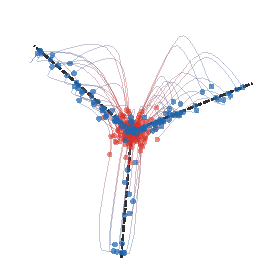
\includegraphics[width=.34\linewidth]{figures/gradflow-mlp-homogeneous-relu--neuron-trajectories.pdf} &
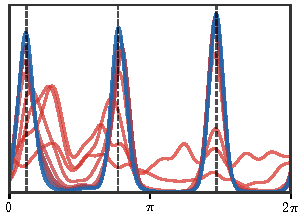
\includegraphics[width=.34\linewidth]{figures/gradflow-mlp-homogeneous-relu--direction-histogram.pdf}
\end{tabular}
\caption{Mean-field training of a homogeneous two-layer model as transport in neuron space. The left panel shows the Wasserstein particle gradient flow in the reduced homogeneous coordinates $(|u|v_1,|u|v_2)$, with black dashed rays marking the teacher directions. The right panel shows the weighted angular density along a front-loaded sequence of times, colored from red to blue, so that the early concentration of neuron directions is visible. The display follows the rendering of the auxiliary MLP experiment but keeps only the $W_2$ flow, not the spectral-flow comparison.}
\index{two-layer neural network}% strictindex
\index{gradient!flow}% strictindex
\label{fig:gradflow-mlp-homogeneous-relu}
\end{figure}

\paragraph{Classical convexity and stationarity.}
\index{convexity!classical}% strictindex
\index{stationarity}% strictindex
Before using the specific homogeneity mechanism of Chizat and Bach, it is useful to isolate a simpler convex-analytic principle behind many mean-field arguments. Consider an energy of the form
\[
	f(\alpha)
	=
	\frac12\iint k(x,x')\d\alpha(x)\d\alpha(x')
	+
	\int V(x)\d\alpha(x)
	+C,
\]
on probability measures over a parameter domain. Assume that the quadratic part is convex in the classical sense, namely convex for the affine structure of measures:
\index{probability measure}% strictindex
\[
	Q((1-s)\alpha+s\beta)\leq (1-s)Q(\alpha)+sQ(\beta),
	\qquad
	Q(\alpha)=\frac12\iint k\d\alpha\d\alpha.
\]
This is ordinary convexity of the functional on the convex set of measures, not displacement convexity along $\Wass_2$ geodesics.
\index{convexity!along geodesics}% strictindex
\index{displacement convexity}% strictindex

\begin{prop}[Affine convexity and stationary positive densities]\label{prop-classical-convex-stationary}
\index{convexity!classical}% strictindex
\index{stationary density}% strictindex
	Let $\Omega\subset\RR^d$ be connected, let $f=Q+\int V\,\d\alpha+C$ be as above on $\Pp(\Omega)$, and assume that $Q$ is classically convex. Suppose that a Wasserstein gradient flow $\alpha_t$ of $f$ converges to $\alpha_\infty=\rho_\infty\d x$, where $\rho_\infty>0$ almost everywhere on $\Omega$, and that $\inf_{t\geq0}f(\alpha_t)>-\infty$. Assume that $\delta f(\alpha_\infty)\in C^1(\Omega)$ and that the squared Wasserstein slope is lower semicontinuous along the convergence, in the sense that
\index{stationary condition}% strictindex
\index{first variation}% strictindex
\index{stationarity}% strictindex
\index{Wasserstein!gradient}% strictindex
\index{gradient!flow}% strictindex
\index{Wasserstein!gradient flow}% strictindex
	\[
		\int_\Omega\norm{\nabla\delta f(\alpha_\infty)}^2\d\alpha_\infty
		\leq
		\liminf_{n\to\infty}
		\int_\Omega\norm{\nabla\delta f(\alpha_{t_n})}^2\d\alpha_{t_n}
	\]
	whenever $t_n\to\infty$. Then $\alpha_\infty$ is a global minimizer of $f$.
\index{global!minimizer}% strictindex
\end{prop}
\begin{proof}
	The energy-dissipation identity and the lower bound on $f$ along the convergent trajectory imply
\index{gradient!flow}% strictindex
	\[
		\int_0^\infty\int_\Omega
		\norm{\nabla\delta f(\alpha_t)}^2\d\alpha_t\d t<+\infty.
	\]
	Hence there exists $t_n\to\infty$ for which the inner integral tends to zero. Lower semicontinuity gives
	\[
		\int_\Omega\norm{\nabla\delta f(\alpha_\infty)}^2\d\alpha_\infty=0.
	\]
	Because $\rho_\infty>0$ almost everywhere and $\nabla\delta f(\alpha_\infty)$ is continuous, this gradient vanishes throughout $\Omega$. Connectedness implies that $\delta f(\alpha_\infty)$ is constant, and therefore
	\(
	\int_\Omega\delta f(\alpha_\infty)\d(\beta-\alpha_\infty)=0
	\)
	for every $\beta\in\Pp(\Omega)$. Classical convexity of $f$ in the affine variable $\alpha$ gives the usual subgradient inequality
\index{subgradient inequality}% strictindex
\index{first variation}% strictindex
\index{convexity!classical}% strictindex
	\[
		f(\beta)\geq f(\alpha_\infty)
		+
		\int \delta f(\alpha_\infty)\d(\beta-\alpha_\infty)
		=f(\alpha_\infty).
	\]
	Thus no competitor has smaller energy. Strict positivity is essential: without it, stationarity controls the first variation only on the support explored by the limiting measure. For square-loss two-layer mean-field models, \eqref{eq-mlp-square-loss-quadratic-linear} is exactly of this quadratic-plus-linear form, and positive semidefiniteness of the induced kernel $k$ is the classical convexity assumption.
\index{linear!form}% strictindex
\index{two-layer neural network}% strictindex
\index{convexity!classical}% strictindex
\index{classical convexity}% strictindex
\end{proof}

The convergence theory then separates two regimes. Chizat and Bach prove global convergence for the unregularized, noiseless Wasserstein flow of positively homogeneous models~\cite{ChizatBach2018OverparameterizedOT}. Mei, Montanari and Nguyen prove convergence for the noisy, regularized dynamics~\cite{MeiMontanariNguyen2018MeanFieldNN}: at the PDE level the noise adds a diffusion, or Laplacian, term, so an initially singular neuron law is immediately smoothed and acquires a density. Rotskoff and Vanden-Eijnden emphasize the parameters-as-particles interpretation, long-time convergence and asymptotic error scaling with the network width~\cite{RotskoffVandenEijnden2018Trainability}. The following formal statement isolates the noiseless Chizat--Bach mechanism and ignores the technical issues due to ReLU non-smoothness, support propagation and compactness.
\index{noisy gradient descent}% strictindex
\index{interacting particle system}% strictindex

\begin{prop}[Formal global optimality for two-homogeneous mean-field flows]\label{prop-formal-chizat-bach}
\index{global!optimality}% strictindex
	Assume that the feature is positively two-homogeneous in the neuron variable,
\index{neuron}% strictindex
	\[
		\psi(\lambda x,z)=\lambda^2\psi(x,z)
		\qquad(\lambda>0),
	\]
	and that $f(\alpha)=J(G_\alpha)$ with $J$ convex and differentiable as a functional of the predictor. Let $\alpha$ be a smooth stationary point of the Wasserstein flow, so that $\nabla_x\delta f(\alpha)(x)=0$ on $\supp(\alpha)$. Assume also full directional support: for every unit direction $\omega$, the support of $\alpha$ intersects the ray $\{\lambda\omega:\lambda>0\}$. Then $\alpha$ is a global minimizer of $f$ over the mean-field model class.
\index{stationarity}% strictindex
\index{global!minimizer}% strictindex
\end{prop}
\begin{proof}
	Choose the first-variation representative
	\[
		h_\alpha(x)=\delta f(\alpha)(x)
		=
		\left\langle \nabla J(G_\alpha),\psi(x,\cdot)\right\rangle_\zeta .
	\]
	Additive constants in first variations do not affect the Wasserstein gradient or first-order inequalities between probability measures; this normalization is useful because it inherits the homogeneity of $\psi$. By two-homogeneity of $\psi$, one has
	\[
		h_\alpha(\lambda x)=\lambda^2h_\alpha(x),
		\qquad \lambda>0.
	\]
	Taking \(x=0\) and any \(\lambda\neq1\) in this identity gives \(h_\alpha(0)=0\). We first record that stationarity forces \(h_\alpha\) to vanish on \(\supp(\alpha)\). Indeed, if \(x=r\omega\in\supp(\alpha)\) with \(r>0\) and \(\norm{\omega}=1\), then
	\[
		0=\dotp{\nabla h_\alpha(r\omega)}{\omega}
		=\frac{\d}{\d s}h_\alpha(s\omega)\bigg|_{s=r}
		=2r h_\alpha(\omega),
	\]
	so \(h_\alpha(\omega)=0\), and hence \(h_\alpha(x)=r^2h_\alpha(\omega)=0\). The case \(x=0\) has already been covered, so \(h_\alpha=0\) on \(\supp(\alpha)\) and \(\int h_\alpha\,\d\alpha=0\).

	We now argue by contradiction. Suppose that a competitor \(\beta\) satisfies \(f(\beta)<f(\alpha)\). Since
	\[
		G_\beta-G_\alpha
		=
		\int \psi(x,\cdot)\d(\beta-\alpha)(x),
	\]
	convexity of \(J\) gives
	\[
		f(\beta)-f(\alpha)
		\geq
		\int h_\alpha(x)\d(\beta-\alpha)(x).
	\]
	The left-hand side is negative, while \(\int h_\alpha\,\d\alpha=0\), so \(\int h_\alpha\,\d\beta<0\). Since \(h_\alpha(0)=0\), this strict negativity must occur away from the origin: there exists a nonzero point \(x=r\omega\) with \(r>0\), \(\norm{\omega}=1\), and \(h_\alpha(x)<0\). Equivalently \(h_\alpha(\omega)=h_\alpha(x)/r^2<0\). By full directional support, there is \(r_\omega>0\) such that \(r_\omega\omega\in\supp(\alpha)\). At this support point,
	\[
		\dotp{\nabla h_\alpha(r_\omega\omega)}{\omega}
		=
		2r_\omega h_\alpha(\omega)
		<0,
	\]
	which contradicts the stationarity condition \(\nabla h_\alpha=0\) on \(\supp(\alpha)\). Thus no competitor has smaller risk.

	The rigorous Chizat--Bach theorem replaces the full directional support assumption by propagation and overparameterization hypotheses ensuring that any negative first-variation direction is represented by the evolving support. The same radial-derivative contradiction, applied after this support-propagation step, then rules out non-optimal stationary limits.
\index{stationarity}% strictindex
\end{proof}

\section{Conditional Wasserstein Training of Infinite ResNets}
\label{sec-conditional-wasserstein-resnets}
\index{conditional!optimal transport}% strictindex
\index{conditional!Wasserstein distance}% strictindex
\index{ResNet}% strictindex
Residual networks learn small residual updates around the identity~\cite{HeZhangRenSun2016ResNet}. This makes depth behave like time: very deep residual architectures can be interpreted as discretizations of differential equations, a viewpoint developed in stable architectures, neural ODEs and mean-field optimal-control models of deep learning~\cite{HaberRuthotto2017StableArchitectures,LuZhongLiDong2018BeyondFiniteLayers,Chen2018NeuralODE,EHanLi2019MeanFieldDeepLearning}. The conditional-OT formulation of Barboni, Peyr\'e and Vialard~\cite{BarboniPeyreVialard2024ConditionalResNets} adds the width mean-field limit to this continuous-depth picture. It belongs to a broader conditional-transport literature, including fibered gradient flows~\cite{PeszekPoyato2023FiberedOptimalTransport}, conditional optimal transport on function spaces~\cite{HosseiniHsuTaghvaei2023ConditionalFunctionSpaces}, conditional Wasserstein distances for Bayesian OT flow matching~\cite{ChemseddineHagemannSteidlWald2024ConditionalWasserstein}, and dynamic conditional OT through simulation-free flows~\cite{KerriganMiglioriniSmyth2024DynamicConditionalOT}. The point of the construction is to keep track of two independent symmetries: neurons can be relabelled inside each layer, but mass should not move from one depth to another. Conditional Wasserstein geometry implements exactly this rule. It transports neurons fiber by fiber in parameter space, while the depth variable remains fixed.

We follow the three limiting levels of the model. A finite ResNet is first a labelled particle system arranged by layers. Sending the width to infinity turns each layer into a probability law of neurons. Sending the depth step to zero then turns the sequence of layer laws into a conditional measure indexed by depth, on which training becomes a Wasserstein gradient flow.

\paragraph{Finite-depth finite-width ResNets.}
The starting point is the ordinary architecture: depth is discrete, width is finite, and each layer carries a labelled collection of neurons. Fix a parameter space $\Theta\subset\RR^q$, a residual feature $\psi:\Theta\times\RR^d\to\RR^d$, a data law $\zeta$ on input-label pairs $(z,y)$, and a loss $\ell$. With $L$ layers, step size $\tau=1/L$, widths $n_r$, and parameters $\theta_{r,i}\in\Theta$, a finite ResNet is the composition of the residual updates
\begin{equation}\label{eq-finite-resnet}
	z_{r+1}
	=
	z_r+\tau G_{r,n_r}(z_r),
	\qquad
	G_{r,n_r}(z)
	\eqdef
	\frac1{n_r}\sum_{i=1}^{n_r}\psi(\theta_{r,i},z),
	\qquad
	z_0=z,\qquad r=0,\ldots,L-1.
\end{equation}
The associated population loss, with $n=(n_0,\ldots,n_{L-1})$, is
\[
	f_{L,n}((\theta_{r,i})_{r,i})
	=
	\int \ell(z_L^{\theta}(z),y)\d\zeta(z,y).
\]
Equivalently, each layer carries an empirical neuron law
\[
	\alpha_r
	=
	\frac1{n_r}\sum_{i=1}^{n_r}\delta_{\theta_{r,i}},
	\qquad
	G_{r,n_r}(z)
	=
	\int_\Theta\psi(\theta,z)\d\alpha_r(\theta).
\]
Thus a finite ResNet is already a discrete conditional measure on depth and neuron space,
\[
	\alpha^{L,n}(\d s,\d\theta)
	=
	\frac1L\sum_{r=0}^{L-1}\delta_{s_r}(\d s)\alpha_r(\d\theta),
	\qquad
	s_r=r/L,
\]
whose marginal on the depth variable is the discrete measure $\lambda_L=L^{-1}\sum_{r=0}^{L-1}\delta_{s_r}$.
\index{empirical!measure}% strictindex
\index{neuron}% strictindex

\paragraph{Finite-depth mean-field limit.}
The first mean-field limit removes neuron labels inside each fixed layer. The residual depth grid stays discrete, but the widths tend to infinity. Each empirical law $\alpha_r$ is replaced by an arbitrary probability measure in $\Pp_2(\Theta)$, and each residual block becomes a mean-field residual block
\[
	z_{r+1}
	=
	z_r+\tau G_{\alpha_r}(z_r),
	\qquad z_0=z,
	\qquad
	G_{\alpha_r}(z)
	\eqdef
	\int_\Theta\psi(\theta,z)\d\alpha_r(\theta).
\]
The loss becomes a functional of the finite family of layer measures,
\[
	f_L(\alpha_0,\ldots,\alpha_{L-1})
	=
	\int \ell(z_L^\alpha(z),y)\d\zeta(z,y).
\]
This is the finite-depth conditional Wasserstein setting with condition marginal $\lambda_L$: each fiber $s_r$ carries a Wasserstein geometry on neuron laws.

\paragraph{Continuous-depth conditional geometry.}
The second limit turns the layer index into a conditioning variable. The model is no longer described by one neuron law, nor even by a finite list of them, but by a family of neuron laws indexed by depth. The state is therefore a conditional probability law
\[
	\alpha(\d s,\d\theta)=\alpha_s(\d\theta)\d s,
\]
or, equivalently, a probability measure on $[0,1]\times\Theta$ whose first marginal is Lebesgue measure. The general conditional Wasserstein distance is defined in Section~\ref{sec-conditional-wasserstein-distances}. Here the condition is continuous depth, $s\in[0,1]$, the condition law is $\lambda(\d s)=\d s$, and the fiber space is the neuron parameter space $\Theta$. For two conditional neuron laws $\alpha(\d s,\d\theta)=\alpha_s(\d\theta)\d s$ and $\beta(\d s,\d\theta)=\beta_s(\d\theta)\d s$, the relevant distance is the depthwise quadratic Wasserstein metric
\begin{equation}\label{eq-resnet-depth-wasserstein}
	\Wass_{2,\lambda}^2(\alpha,\beta)
	=
	\int_0^1\Wass_2^2(\alpha_s,\beta_s)\d s.
\end{equation}
It compares neurons only at the same depth: transport in $\theta$ is allowed fiber by fiber, while mass is not transported between layers.

\paragraph{Infinite-depth mean-field ResNet.}
Once depth is continuous, the forward pass is a controlled ODE and the control is the conditional neuron law. A mean-field infinite-depth and infinite-width ResNet is described by a measurable family $s\mapsto\alpha_s\in\Pp_2(\Theta)$. Each slice is the neuron law of one infinitesimal residual block, and the feature $\psi(\theta,z)$ now acts as a vector field on the state variable. The forward pass is
\begin{equation}\label{eq-mean-field-resnet-forward}
	\partial_s z_s
	=
	G_{\alpha_s}(z_s)
	\eqdef
	\int_\Theta \psi(\theta,z_s)\d\alpha_s(\theta),
	\qquad z_0=z.
\end{equation}
The population risk is
\[
	f_{\mathrm{Res}}(\alpha)
	=
	\int \ell(z_1^\alpha(z),y)\d\zeta(z,y).
\]
Under the usual regularity assumptions ensuring well-posedness of the ODE, this defines a functional on the conditional Wasserstein space.

\paragraph{Conditional Wasserstein gradient flow.}
Training is now steepest descent for an objective on conditional laws. More generally, let $(S,\lambda)$ be a probability space and let $f$ be a differentiable functional on measures $\alpha(\d s,\d\theta)=\alpha_s(\d\theta)\lambda(\d s)$ with fixed first marginal $\lambda$. For signed perturbations $\xi(\d s,\d\theta)=\xi_s(\d\theta)\lambda(\d s)$ satisfying $\int_\Theta\d\xi_s=0$ for $\lambda$-a.e. $s$, we use the fiberwise first-variation convention
\[
	\frac{\d}{\d\varepsilon}f(\alpha+\varepsilon\xi)\bigg|_{\varepsilon=0}
	=
	\int_S\int_\Theta \frac{\delta f}{\delta\alpha_s}(\alpha)(\theta)\d\xi_s(\theta)\d\lambda(s).
\]
The formal conditional Wasserstein gradient flow is the family of continuity equations
\begin{equation}\label{eq-conditional-resnet-gradient-flow}
	\partial_t\alpha_{t,s}
	+\diverg_\theta(\alpha_{t,s}v_{t,s})=0,
	\qquad
	v_{t,s}(\theta)
	=
	-\nabla_\theta\frac{\delta f}{\delta\alpha_s}(\alpha_t)(\theta),
\end{equation}
for $\lambda$-a.e. condition $s$, whenever the first variation is differentiable in the parameter variable. In the ResNet case one takes $f=f_{\mathrm{Res}}$ and $S=[0,1]$. The equation is fiberwise in its transport geometry, but not decoupled as a training dynamics: changing $\alpha_s$ affects the terminal loss through the forward ODE and the corresponding adjoint equation. Thus each depth performs a Wasserstein steepest descent in its own neuron space, while all depths interact through the state trajectory.
\index{first variation}% strictindex
\index{Wasserstein!gradient flow}% strictindex

\paragraph{Particle discretization and layerwise matching.}
The finite network is recovered by discretizing both the condition variable and the fiber measures. With the discrete depth marginal $\lambda_L$, finite-depth finite-width ResNets are particle approximations of the conditional flow above. If two networks have the same depth grid and the same widths, and if their empirical layer laws are
\[
	\alpha_r=\frac1{n_r}\sum_{i=1}^{n_r}\delta_{\theta_{r,i}},
	\qquad
	\beta_r=\frac1{n_r}\sum_{i=1}^{n_r}\delta_{\theta'_{r,i}},
\]
then their squared conditional distance is
\[
	\Wass_{2,\lambda_L}^2(\alpha^{L,n},\beta^{L,n})
	=
	\frac1L\sum_{r=0}^{L-1} \Wass_2^2(\alpha_r,\beta_r).
\]
Keeping neuron labels fixed gives the labelled parameter distance
\[
	\frac1L\sum_{r=0}^{L-1}\frac1{n_r}
	\sum_{i=1}^{n_r}\norm{\theta_{r,i}-\theta'_{r,i}}^2,
\]
which corresponds to a particular feasible coupling and therefore upper bounds the squared conditional Wasserstein distance. Optimizing over permutations inside each equal-weight layer gives the Wasserstein matching term above. In this sense, the shallow mean-field flow is the one-fiber case, whereas infinitely deep ResNets require a continuum of Wasserstein flows indexed by depth and coupled through the network state.
\index{continuous!depth}% strictindex
\index{residual network}% strictindex
\index{mean-field neural network}% strictindex
\index{Wasserstein!gradient flow}% strictindex

\section{Functional Inequalities via Optimal Transport}
\index{functional inequality}% strictindex
\index{isoperimetric inequality}% strictindex
\index{transport!inequality}% strictindex

Optimal transport is also a proof technique for sharp inequalities. The common mechanism is simple: push one density to another by a monotone or Brenier map, interpolate along the transport rays, and convert convexity of the determinant, entropy, or the cost into an integral inequality. This section records a few representative examples. To keep the presentation readable, the proofs are written in the smooth Euclidean setting; the usual regularization and approximation arguments give the standard Borel or Sobolev versions. The transport viewpoint is developed systematically in McCann's displacement convexity principle, the Riemannian interpolation inequalities of Cordero-Erausquin, McCann and Schmuckenschl\"ager, and Villani's account of concentration and functional inequalities~\cite{mccann1997convexity,cordero2001riemannian,Villani09}.
\index{Brenier!map}% strictindex
\index{displacement convexity}% strictindex

\paragraph{Brunn--Minkowski and isoperimetry.}
\index{Brunn-Minkowski inequality}% strictindex
\index{isoperimetric inequality}% strictindex
The most geometric use of OT is to prove that transporting two uniform measures and looking at the interpolated support increases volume at least concavely. The perimeter inequality is then obtained by differentiating this volume estimate after adding a small ball.

\begin{prop}[Brunn--Minkowski and Euclidean isoperimetry]\label{prop-ot-brunn-minkowski-isoperimetric}
	Let $A,B\subset\RR^d$ be bounded Borel sets with positive Lebesgue measure. For $t\in[0,1]$, set
	\[
		(1-t)A+tB\eqdef\{(1-t)x+ty\;:\;x\in A,\ y\in B\}.
	\]
	Then
	\[
		\mathrm{Vol}((1-t)A+tB)^{1/d}
		\geq
		(1-t)\mathrm{Vol}(A)^{1/d}
		+
		t\,\mathrm{Vol}(B)^{1/d}.
	\]
	Consequently, if $A$ is smooth and bounded and $\omega_d=\mathrm{Vol}(B_1)$, then
	\[
		\mathrm{Per}(A)
		\geq
		d\,\omega_d^{1/d}\mathrm{Vol}(A)^{(d-1)/d}.
	\]
\end{prop}

\begin{proof}
	We first give the argument for regular sets, the general Borel case following by approximation from inside and outside. Let $\alpha$ and $\beta$ be the uniform probability measures on $A$ and $B$, and let $T=\nabla\phi$ be the Brenier map with $T_\sharp\alpha=\beta$. The interpolating map $T_t=(1-t)\Id+tT$ sends $\alpha$ to a measure $\alpha_t$ supported in $(1-t)A+tB$. At points where $T$ is differentiable,
	\[
		\det DT_t
		=
		\det((1-t)\Id+tDT).
	\]
	Since $DT$ is symmetric positive semidefinite and $\det^{1/d}$ is concave on the positive semidefinite cone,
	\[
		\det(DT_t)^{1/d}
		\geq
		(1-t)+t\det(DT)^{1/d}.
	\]
	The change-of-variables identity for the uniform measures gives $\det(DT)=\mathrm{Vol}(B)/\mathrm{Vol}(A)$ almost everywhere. Hence the density $\rho_t$ of $\alpha_t$ satisfies
	\[
		\rho_t^{-1/d}
		\geq
		(1-t)\mathrm{Vol}(A)^{1/d}
		+
		t\mathrm{Vol}(B)^{1/d}.
	\]
	This means that $\rho_t\leq c_t^{-d}$ on its support, where $c_t=(1-t)\mathrm{Vol}(A)^{1/d}+t\mathrm{Vol}(B)^{1/d}$. Since $\alpha_t$ has total mass one and is supported in $(1-t)A+tB$, this gives $\mathrm{Vol}((1-t)A+tB)\geq c_t^d$, which is the displayed Brunn--Minkowski inequality.
\index{Brunn-Minkowski inequality}% strictindex

	For isoperimetry, apply Brunn--Minkowski with $B=B_1$ and write $A+\epsilon B_1$ for the parallel set. Then
\index{isoperimetric inequality}% strictindex
	\[
		\mathrm{Vol}(A+\epsilon B_1)^{1/d}
		\geq
		\mathrm{Vol}(A)^{1/d}+\epsilon\omega_d^{1/d}.
	\]
	Using $\mathrm{Vol}(A+\epsilon B_1)=\mathrm{Vol}(A)+\epsilon\,\mathrm{Per}(A)+o(\epsilon)$ and differentiating at $\epsilon=0$ yields the claimed perimeter bound.
\end{proof}

Figure~\ref{fig:gradflow-brunn-minkowski-ot} isolates the determinant-concavity step in the special case where the optimal map is affine.

\begin{figure}
\centering
\setlength{\tabcolsep}{1.5pt}
\begin{tabular}{@{}cccccc@{}}
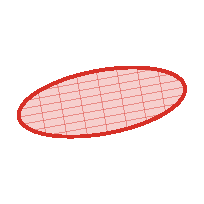
\includegraphics[width=.118\linewidth]{figures/gradflow-brunn-minkowski-ot--ellipse-t000.pdf} &
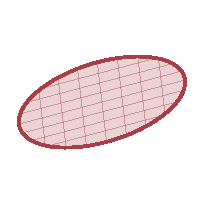
\includegraphics[width=.118\linewidth]{figures/gradflow-brunn-minkowski-ot--ellipse-t025.pdf} &
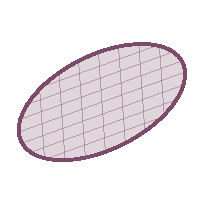
\includegraphics[width=.118\linewidth]{figures/gradflow-brunn-minkowski-ot--ellipse-t050.pdf} &
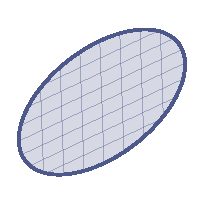
\includegraphics[width=.118\linewidth]{figures/gradflow-brunn-minkowski-ot--ellipse-t075.pdf} &
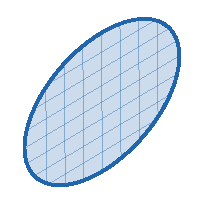
\includegraphics[width=.118\linewidth]{figures/gradflow-brunn-minkowski-ot--ellipse-t100.pdf} &
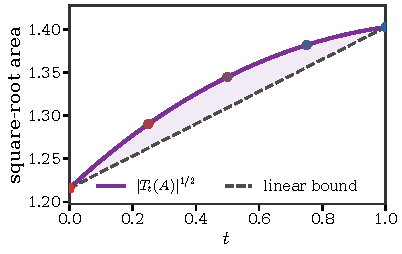
\includegraphics[width=.265\linewidth]{figures/gradflow-brunn-minkowski-ot--area-concavity.pdf} \\[-.1em]
\small $t=0$ & \small $t=.25$ & \small $t=.5$ & \small $t=.75$ & \small $t=1$ & \small area inequality
\end{tabular}
\caption{Brunn--Minkowski through an affine optimal-transport interpolation between two ellipses. For ellipses, the Brenier map is affine, so the transported support $T_t(A)$ remains an ellipse and its area is computed exactly from the determinant of $(1-t)\Id+tDT$. The right panel shows that $|T_t(A)|^{1/2}$ lies above the linear interpolation of the endpoint square-root areas, which is the two-dimensional determinant concavity behind the proof of Brunn--Minkowski.}
\label{fig:gradflow-brunn-minkowski-ot}
\index{Brunn-Minkowski inequality}% strictindex
\index{Brenier!map}% strictindex
\end{figure}

\paragraph{Pr\'ekopa--Leindler.}
\index{Prekopa@Pr\'ekopa!Leindler inequality}% strictindex
\index{functional inequality}% strictindex
The functional analogue of Brunn--Minkowski replaces sets by densities. The transport proof is the same argument with the Jacobian no longer constant.

\begin{prop}[Pr\'ekopa--Leindler inequality]\label{prop-ot-prekopa-leindler}
	Let $u,v,w:\RR^d\to[0,+\infty)$ be integrable, and let $t\in[0,1]$. Assume that
	\[
		w((1-t)x+ty)\geq u(x)^{1-t}v(y)^t
		\qquad
		\text{for all }x,y\in\RR^d.
	\]
	Then
	\[
		\int_{\RR^d} w
		\geq
		\left(\int_{\RR^d}u\right)^{1-t}
		\left(\int_{\RR^d}v\right)^t .
	\]
\end{prop}

\begin{proof}
	Set $U=\int u$ and $V=\int v$, and assume $U,V>0$. Let $\alpha=(u/U)\d x$ and $\beta=(v/V)\d x$, and let $T$ be the Brenier map from $\alpha$ to $\beta$. Put $T_t=(1-t)\Id+tT$. The change of variables gives
	\[
		\int w
		\geq
		\int w(T_t(x))\det(DT_t(x))\d x .
	\]
	By the assumption on $w$ and by $\det((1-t)\Id+tDT)\geq\det(DT)^t$ for positive semidefinite $DT$,
	\[
		\int w
		\geq
		\int u(x)^{1-t}v(T(x))^t\det(DT(x))^t\d x.
	\]
	Since $T_\sharp\alpha=\beta$, the Monge--Amp\`ere identity gives
	\[
		\det(DT(x))=\frac{u(x)V}{v(T(x))U}
	\]
	almost everywhere. Substitution yields
	\[
		\int w
		\geq
		\left(\frac{V}{U}\right)^t\int u(x)\d x
		=
		U^{1-t}V^t.
	\]
	Approximation removes the smoothness and positivity assumptions.
\end{proof}

\paragraph{Gaussian logarithmic Sobolev inequality.}
\index{logarithmic Sobolev inequality}% strictindex
\index{Gaussian!measure}% strictindex
Transport also gives a short proof of the sharp Gaussian logarithmic Sobolev inequality. The key point is that the Jacobian equation for the Brenier map can be bounded by $\log\det A\leq\tr(A-\Id)$, and Gaussian integration by parts converts the trace term into a Fisher information.

\begin{prop}[Gaussian logarithmic Sobolev inequality]\label{prop-gaussian-log-sobolev-ot}
\index{Fisher information}% strictindex
	Let $\gamma_d$ be the standard Gaussian measure on $\RR^d$. If $\rho$ is a smooth positive probability density with respect to $\gamma_d$, has sufficient decay, and $\int \rho\,\d\gamma_d=1$, then
	\[
		\mathrm{Ent}_{\gamma_d}(\rho)
		\eqdef
		\int \rho\log \rho\,\d\gamma_d
		\leq
		\frac12\int \frac{\norm{\nabla \rho}^2}{\rho}\,\d\gamma_d.
	\]
\end{prop}

\begin{proof}
	Let $\al=\rho\gamma_d$, and let $T=\nabla\phi$ be the Brenier map with $T_\sharp\al=\gamma_d$. Write $T(x)=x+\theta(x)$. The Monge--Amp\`ere equation reads
	\[
		\rho(x)e^{-\norm{x}^2/2}
		=
		e^{-\norm{T(x)}^2/2}\det(DT(x)).
	\]
	Thus
	\[
		\log \rho(x)
		=
		-\dotp{x}{\theta(x)}
		-\frac12\norm{\theta(x)}^2
		+
		\log\det(\Id+D\theta(x)).
	\]
	Since $DT$ is positive semidefinite, $\log\det(\Id+D\theta)\leq\tr(D\theta)=\diverg\theta$. Multiplying by $\rho$ and integrating with respect to $\gamma_d$ gives
	\[
		\mathrm{Ent}_{\gamma_d}(\rho)
		\leq
		\int \rho(\diverg\theta-\dotp{x}{\theta})\,\d\gamma_d
		-\frac12\int \rho\norm{\theta}^2\,\d\gamma_d.
	\]
	Gaussian integration by parts gives
	\[
		\int \rho(\diverg\theta-\dotp{x}{\theta})\,\d\gamma_d
		=
		-\int\dotp{\nabla \rho}{\theta}\,\d\gamma_d.
	\]
	Completing the square pointwise,
	\[
		-\dotp{\nabla \rho}{\theta}-\frac12 \rho\norm{\theta}^2
		\leq
		\frac12\frac{\norm{\nabla \rho}^2}{\rho}.
	\]
	This proves the inequality. The general Sobolev-class statement follows by approximation.
\end{proof}

\paragraph{Talagrand's transport-entropy inequality.}
\index{Talagrand inequality}% strictindex
\index{transport-entropy inequality}% strictindex
The same Jacobian estimate gives the sharp quadratic transport-entropy inequality for the Gaussian. This result is due to Talagrand~\cite{Talagrand1996Transport}; the link with logarithmic Sobolev inequalities and the Otto calculus is one of the starting points of the Otto--Villani theory~\cite{OttoVillani2000Generalization,Villani09}.
\index{logarithmic Sobolev inequality}% strictindex

\begin{prop}[Gaussian \(T_2\) inequality]\label{prop-gaussian-talagrand-t2}
	Let $\al=\rho\gamma_d$ be a probability measure with finite second moment. Then
	\[
		\frac12\Wass_2^2(\al,\gamma_d)
		\leq
		\KL(\al|\gamma_d)
		=
		\int \rho\log \rho\,\d\gamma_d .
	\]
\end{prop}

\begin{proof}
	Assume first that $\rho$ is smooth and positive. Let $T=\nabla\phi$ be the Brenier map with $T_\sharp\gamma_d=\al$, and write $T(x)=x+\theta(x)$. The change of variables gives
	\[
		\rho(T(x))e^{-\norm{T(x)}^2/2}\det(DT(x))
		=
		e^{-\norm{x}^2/2}.
	\]
	Hence
	\[
		\log \rho(T(x))
		=
		\dotp{x}{\theta(x)}
		+
		\frac12\norm{\theta(x)}^2
		-
		\log\det(\Id+D\theta(x)).
	\]
	Using again $\log\det(\Id+D\theta)\leq\diverg\theta$ and integrating with respect to $\gamma_d$,
	\[
		\KL(\al|\gamma_d)
		\geq
		\frac12\int\norm{\theta}^2\,\d\gamma_d
		+
		\int(\dotp{x}{\theta}-\diverg\theta)\,\d\gamma_d.
	\]
	The last integral vanishes by Gaussian integration by parts. Since $T$ is optimal,
	\[
		\int\norm{\theta}^2\,\d\gamma_d=\Wass_2^2(\gamma_d,\al),
	\]
	which proves the claim. Approximation gives the general case.
\end{proof}

\paragraph{The HWI bridge.}
\index{HWI inequality}% strictindex
\index{Fisher information}% strictindex
The previous two Gaussian inequalities are not isolated facts. The HWI inequality of Otto and Villani~\cite{OttoVillani2000Generalization} compares three quantities at once: the entropy \(H\), the Wasserstein distance \(W\), and the Fisher information \(I\). It is one of the cleanest examples where displacement convexity turns into a functional inequality.

\begin{prop}[Otto--Villani HWI inequality]\label{prop-hwi-inequality}
\index{displacement convexity}% strictindex
	Let $\beta=\rho_\beta\d x=e^{-V}\d x/Z$ be a smooth probability measure in $\Pp_2(\RR^d)$, and assume that $\nabla^2 V\succeq \lambda \Id$ for some $\lambda\in\RR$. For an absolutely continuous probability measure $\alpha=\rho_\alpha\d x$ in $\Pp_2(\RR^d)$, define the relative Fisher information
	\[
		\mathcal I(\alpha|\beta)
		\eqdef
		\int \norm{\nabla\log\frac{\rho_\alpha}{\rho_\beta}}^2\,\d\alpha,
	\]
	with the convention $\mathcal I(\alpha|\beta)=+\infty$ if $\alpha$ is not absolutely continuous or if the expression is not defined. Then
	\[
		\KL(\alpha|\beta)
		\leq
		\Wass_2(\alpha,\beta)\sqrt{\mathcal I(\alpha|\beta)}
		-\frac{\lambda}{2}\Wass_2^2(\alpha,\beta).
	\]
\end{prop}

\begin{proof}
	If $\mathcal I(\alpha|\beta)=+\infty$, there is nothing to prove. Assume first that $\rho_\alpha$ is smooth and positive. Let $T$ be the Brenier map from $\alpha$ to $\beta$, set $v=T-\Id$, and let $\alpha_t=((1-t)\Id+tT)_\sharp\alpha$. By Proposition~\ref{prop-basic-geodesic-convexity}, $F(\eta)=\KL(\eta|\beta)$ is $\lambda$-geodesically convex. Thus the one-dimensional function $f(t)=F(\alpha_t)$ satisfies
	\[
		f(1)\geq f(0)+f'(0)+\frac{\lambda}{2}\Wass_2^2(\alpha,\beta).
	\]
	Since $f(1)=F(\beta)=0$, it remains to compute the initial derivative. The continuity equation for the geodesic gives $\partial_t\alpha_t+\nabla\cdot(\alpha_t v_t)=0$ and $v_0=v$. Hence
	\[
		f'(0)
		=
		\int \dotp{\nabla\log\frac{\rho_\alpha}{\rho_\beta}}{v}\,\d\alpha.
	\]
	Therefore
	\[
		\KL(\alpha|\beta)
		\leq
		-\int \dotp{\nabla\log\frac{\rho_\alpha}{\rho_\beta}}{T-\Id}\,\d\alpha
		-\frac{\lambda}{2}\Wass_2^2(\alpha,\beta).
	\]
	Cauchy's inequality and $\int\norm{T-\Id}^2\d\alpha=\Wass_2^2(\alpha,\beta)$ give the announced bound. The general case follows by the standard approximation and lower-semicontinuity of entropy, Fisher information, and $\Wass_2$.
\end{proof}

When $\lambda>0$, Young's inequality $rs-\lambda r^2/2\leq s^2/(2\lambda)$ gives the logarithmic Sobolev estimate $\KL(\alpha|\beta)\leq \mathcal I(\alpha|\beta)/(2\lambda)$. Thus HWI explains why the same curvature assumption controls both the static inequality and the exponential decay of the associated Fokker--Planck flow below.
\index{Fokker-Planck equation@Fokker--Planck equation}% strictindex
\index{logarithmic Sobolev inequality}% strictindex
\index{HWI inequality}% strictindex

Figure~\ref{fig:gradflow-hwi-entropy-decay} shows these inequalities on an exact one-dimensional Ornstein--Uhlenbeck relaxation, where all quantities can be evaluated accurately by grid quadrature and quantile inversion.

\begin{figure}
\centering
\begin{tabular}{@{}ccc@{}}
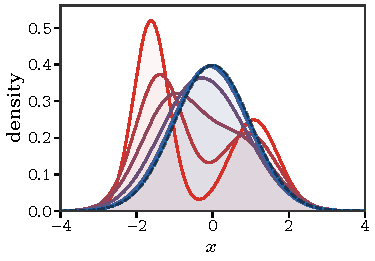
\includegraphics[width=.31\linewidth]{figures/gradflow-hwi-entropy-decay--ou-densities.pdf} &
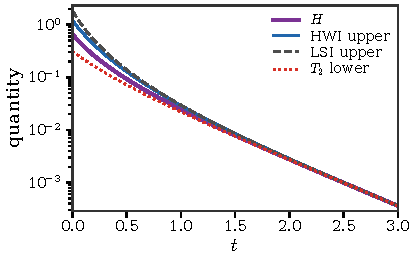
\includegraphics[width=.34\linewidth]{figures/gradflow-hwi-entropy-decay--static-bounds.pdf} &
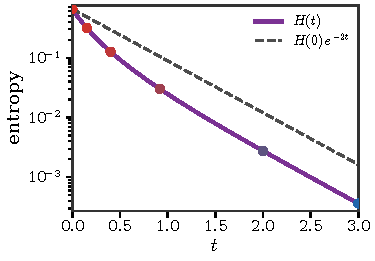
\includegraphics[width=.28\linewidth]{figures/gradflow-hwi-entropy-decay--entropy-decay.pdf} \\[-.1em]
\small Ornstein--Uhlenbeck densities & \small static inequalities & \small entropy decay
\end{tabular}
\caption{Functional inequalities along the Ornstein--Uhlenbeck flow from a one-dimensional Gaussian mixture to the standard Gaussian. The left panel shows the density relaxation, with the Gaussian target as a dashed curve. The middle panel compares the entropy $H=\KL(\alpha_t|\gamma)$ with the HWI upper bound $W\sqrt I-W^2/2$, the logarithmic-Sobolev upper bound $I/2$, and the Talagrand lower bound $W^2/2$. The right panel displays the dynamic consequence of log-Sobolev, namely exponential entropy decay below $H(0)e^{-2t}$.}
\index{Talagrand inequality}% strictindex
\label{fig:gradflow-hwi-entropy-decay}
\index{HWI inequality}% strictindex
\index{logarithmic Sobolev inequality}% strictindex
\index{Ornstein-Uhlenbeck flow}% strictindex
\end{figure}

\paragraph{Back to gradient flows.}
\index{gradient!flow}% strictindex
\index{entropy!dissipation}% strictindex
\index{Fokker-Planck equation@Fokker--Planck equation}% strictindex
Functional inequalities become convergence rates once they are combined with the energy-dissipation identity of a Wasserstein gradient flow. This is why the previous inequalities are not merely static estimates: they quantify relaxation of the Fokker--Planck equation.

\index{HWI inequality}% strictindex
The logarithmic Sobolev assumption below is the same curvature-controlled mechanism as in the HWI discussion. With the convention used here, the standard Gaussian $\gamma=\mathcal N(0,\Id)$ satisfies it with $\lambda=1$, exactly as in Proposition~\ref{prop-gaussian-log-sobolev-ot}. More generally, if $\beta=Z^{-1}e^{-V}\d x$ and $\nabla^2V\succeq\lambda\Id$, then the Bakry--Emery criterion gives the logarithmic Sobolev inequality with constant $\lambda$. Thus the hypothesis covers strongly log-concave targets, and it is the functional-inequality counterpart of the $\lambda$-geodesic convexity of $\KL(\cdot|\beta)$ discussed in Section~\ref{sec-geodesic-convexity}.
\index{logarithmic Sobolev inequality}% strictindex
\index{Bakry-Emery criterion@Bakry--\'Emery criterion}% strictindex
\index{log-concavity}% strictindex

\begin{prop}[Log-Sobolev inequality implies entropy decay]\label{prop-lsi-entropy-decay}
\index{Fokker-Planck equation@Fokker--Planck equation}% strictindex
\index{entropy!decay}% strictindex
	Let $\beta=e^{-V}\d x/Z$ be a smooth probability measure on $\RR^d$. Assume that $\beta$ satisfies the logarithmic Sobolev inequality with constant $\lambda>0$,
	\[
		\KL(\alpha|\beta)
		\leq
		\frac{1}{2\lambda}
		\int \norm{\nabla\log\frac{\d\alpha}{\d\beta}}^2\,\d\alpha .
	\]
	Let $\alpha_t$ solve the Wasserstein gradient flow of $f(\alpha)=\KL(\alpha|\beta)$, namely
	\[
		\partial_t\rho_t
		=
		\nabla\cdot(\rho_t\nabla V)+\Delta\rho_t,
		\qquad
		\alpha_t=\rho_t\d x .
	\]
	Then
	\[
		\KL(\alpha_t|\beta)
		\leq
		e^{-2\lambda t}\KL(\alpha_0|\beta).
	\]
\end{prop}

\begin{proof}
	The first variation of $F$ is $\log(\rho/\rho_\beta)$ up to an additive constant. Along the smooth Wasserstein gradient flow,
	\[
		\frac{\d}{\d t}\KL(\alpha_t|\beta)
		=
		-\int \norm{\nabla\log\frac{\d\alpha_t}{\d\beta}}^2\,\d\alpha_t.
	\]
	The logarithmic Sobolev inequality bounds the Fisher information below by $2\lambda\KL(\alpha_t|\beta)$. Hence
\index{logarithmic Sobolev inequality}% strictindex
	\[
		\frac{\d}{\d t}\KL(\alpha_t|\beta)
		\leq
		-2\lambda\KL(\alpha_t|\beta),
	\]
	and Gronwall's lemma gives the result.
\end{proof}
